\documentclass[a4paper, 12pt, twoside, leqno]{report} %openany, leqno
\usepackage{packagebundle}
% \usepackage{cite}
\pagestyle{plain}
%\setlength{\abovedisplayskip}{0pt}
%\setlength{\belowdisplayskip}{0pt}

% space before and after equations
\expandafter\def\expandafter\normalsize\expandafter{%
    \normalsize%
    \setlength\abovedisplayskip{8pt}%
    \setlength\belowdisplayskip{8pt}%
    \setlength\abovedisplayshortskip{4pt}%
    \setlength\belowdisplayshortskip{4pt}%
}

%\setlength{\parskip}{0pt}
%\setlength{\parindent}{0pt}
\definecolor{myColor}{RGB}{193,225,193}
\newcommand{\B}{\ensuremath{\mathcal{B}}}
\newcommand{\A}{\ensuremath{\mathcal{A}}}
\linespread{1.3}

\patchcmd{\tocchapter}{#1}{\MakeUppercase{#1}}{}{}
\setcounter{tocdepth}{0}

%\renewcommand\@pnumwidth{1em} % <-- depending on the total number of pages
%\patchcmd{\@tocline}
%  {\hfil}
%  {\leaders\hbox{\,.\,}\hfil}
%  {}{}
%\def\l@subsection{\@tocline{2}{0pt}{3.4pc}{5pc}{}}
%\makeatother

%\DeclareRobustCommand{\gobblefour}[5]{}
%\newcommand*{\SkipTocEntry}{\addtocontents{toc}{\gobblefour}}

%\renewcommand{\thesection}{\thechapter.\arabic{section}}
%\renewcommand{\baselinestretch}{1.1}\normalsize

\usetikzlibrary{cd}
\usetikzlibrary{babel}
\usetikzlibrary{knots}

%%%%%%%%%%%%%%%%%%%%%%%%%%%%%%%%%%%%%%%%%%%%%%%%%%%%%%%%%%%%%%%%%%%%%%%%%%%
%%%%% SKEIN RELATIONS
%%%%%%%%%%%%%%%%%%%%%%%%%%%%%%%%%%%%%%%%%%%%%%%%%%%%%%%%%%%%%%%%%%%%%%%%%%%

\makeatletter

% We define separate versions (large and small) for the frames:
\newcommand*\@KP@Large@frame[2]{%
    \setlength\unitlength{\fontdimen 22 #1\tw@}%
    \vrule \@width\z@ \@height 4\unitlength \@depth\tw@\unitlength
    \begin{picture}(6,2)(-3,-1)%
        \def\@KP@Radius     {3}%
        \def\@KP@Hole@radius{.5}% The same value seem adequate for both...
        \def\@KP@Diameter   {6}%
        #2%
    \end{picture}%
}
\newcommand*\@KP@Small@frame[2]{%
    \setlength\unitlength{\fontdimen 22 #1\tw@}%
    \vrule \@width\z@ \@height \thr@@\unitlength \@depth\@ne\unitlength
    \begin{picture}(4,2)(-2,-1)%
        \def\@KP@Radius     {2}%
        \def\@KP@Hole@radius{.5}% ... but let it be customizable too.
        \def\@KP@Diameter   {4}%
        #2%
    \end{picture}%
}

% On the other hand, for the commands that draw the four different shapes, it
% seems that all differences between the small variant and the large one can be
% confined in the following three macros (here, we just declare their name):
\newcommand*\@KP@Radius     {}
\newcommand*\@KP@Hole@radius{}
\newcommand*\@KP@Diameter   {}
%
% The four shapes:
\newcommand*\@KP@Shape@A{%
    \put(0,0){\circle{\@KP@Diameter}}%
}
\newcommand*\@KP@Shape@B{%
    \Line(-\@KP@Radius,\@KP@Radius )(\@KP@Radius,-\@KP@Radius)%
    \Line(-\@KP@Radius,-\@KP@Radius)(-\@KP@Hole@radius,-\@KP@Hole@radius)%
    \Line(\@KP@Radius ,\@KP@Radius )(\@KP@Hole@radius ,\@KP@Hole@radius )%
}
\newcommand*\@KP@Shape@C{%
    \cbezier(-\@KP@Radius,\@KP@Radius )(0,0)(0,0)(\@KP@Radius,\@KP@Radius )%
    \cbezier(-\@KP@Radius,-\@KP@Radius)(0,0)(0,0)(\@KP@Radius,-\@KP@Radius)%
}
\newcommand*\@KP@Shape@D{%
    \cbezier(-\@KP@Radius,-\@KP@Radius)(0,0)(0,0)(-\@KP@Radius,\@KP@Radius)%
    \cbezier(\@KP@Radius ,-\@KP@Radius)(0,0)(0,0)(\@KP@Radius ,\@KP@Radius)%
}
\newcommand*\@KP@Shape@E{%
    \Line(-\@KP@Radius,-\@KP@Radius)(\@KP@Radius,\@KP@Radius)%
    \Line(-\@KP@Hole@radius,\@KP@Hole@radius)(-\@KP@Radius,\@KP@Radius)%
    \Line(\@KP@Radius,-\@KP@Radius)(\@KP@Hole@radius,-\@KP@Hole@radius)%
}
\newcommand*\@KP@Shape@F{%
    \Line(-\@KP@Radius,\@KP@Radius )(\@KP@Radius,-\@KP@Radius)%
    \Line(-\@KP@Radius,-\@KP@Radius)(\@KP@Radius,\@KP@Radius)%
}  
\newcommand*\@KP@Shape@Z{%
    \Line(-\@KP@Radius,-\@KP@Radius)(\@KP@Radius,\@KP@Radius)%
    \Line(-\@KP@Hole@radius,\@KP@Hole@radius)(-\@KP@Radius,\@KP@Radius)%
    \Line(\@KP@Radius,-\@KP@Radius)(-\@KP@Hole@radius,\@KP@Hole@radius)%
}
\newcommand*\@KP@Atomic@mathpalette[1]{%
    \mathinner{% or "\mathord"?
        % Note that a new level of grouping has just been entered (p. 290).
        % \color{gray}% not used, for now
        \mathchoice{%
            \linethickness{.6\p@}% Tip: use thicker lines if you decide to 
                                 % revert to using gray.
            \@KP@Large@frame \textfont {#1}%
        }{%
            \linethickness{.4\p@}% adjustable
            \@KP@Small@frame \textfont {#1}%
        }{%
            \linethickness{.3\p@}% adjustable
            \@KP@Small@frame \scriptfont {#1}%
        }{%
            \linethickness{.2\p@}% adjustable
            \@KP@Small@frame \scriptscriptfont {#1}%
        }%
    }%
}

% User-level commands:
\newcommand*\KPA{\@KP@Atomic@mathpalette \@KP@Shape@A}
\newcommand*\KPB{\@KP@Atomic@mathpalette \@KP@Shape@B}
\newcommand*\KPC{\@KP@Atomic@mathpalette \@KP@Shape@C}
\newcommand*\KPD{\@KP@Atomic@mathpalette \@KP@Shape@D}
\newcommand*\KPE{\@KP@Atomic@mathpalette \@KP@Shape@E}
\newcommand*\KPF{\@KP@Atomic@mathpalette \@KP@Shape@F}
\newcommand*\KPZ{\@KP@Atomic@mathpalette \@KP@Shape@Z}

\makeatother

%%%%%%%%%%%%%%%%%%%%%%%%%%%%%%%%%%%%%%%%%%%%%%%%%%%%%%%%%%%%%%%%%%%%%%%
%%%%%%%%%%%%% OTHER KNOTS, TANGLES
%%%%%%%%%%%%%%%%%%%%%%%%%%%%%%%%%%%%%%%%%%%%%%%%%%%%%%%%%%%%%%%%%%%%%%%

\newcommand*\PKINK{
\begin{tikzpicture}
\begin{knot}[
  consider self intersections,
  flip crossing = 1,
]
\strand (0,0) .. controls +(3,1) and +(-3,1) .. (1,0);
\end{knot}
\end{tikzpicture}
}

\newcommand*\NKINK{
\begin{tikzpicture}
\begin{knot}[
  consider self intersections,
]
\strand (0,0) .. controls +(3,1) and +(-3,1) .. (1,0);
\end{knot}
\end{tikzpicture}
}

\newcommand*\ARC{
\begin{tikzpicture}
\begin{knot}[]
\strand (0,0) .. controls +(3,1) and +(-3,1) .. (1,0);
\end{knot}
\end{tikzpicture}
}

\geometry{
 a4paper,
 left=1.25in,
 right=1in,
 top=1in,
 bottom=1in
}

\begin{document}
\date{}

% Use '\thispagestyle{empty}' to ensure that this page
% is not counted in page numbering.
\thispagestyle{empty}

% Set required margin widths for first few pages.
\newgeometry{top = 2.5in, left = 1.25in, right = 1in, bottom = 1in}
\begin{titlepage}

\begin{center}
    \LARGE
    \textbf{A treatise of the Jones polynomial}

    \vspace{1cm}
    \Large
    \textbf{Huidrom Ronald Mangang}
    \vspace{1cm}
    
    \large
    \textit{A dissertation submitted for the partial fulfilment of
    BS-MS dual degree in Science}
    
    \vspace{3.5cm}

    \includegraphics[trim={5mm 5mm 5mm 5mm},clip,width=8cm]{images/HighResolutionLogo.jpg}

    \large
    \textbf{Indian Institute of Science Education and Research, Mohali}\\
    \large
    \textbf{May 2024}
\end{center}

\end{titlepage}

% Use '\thispagestyle{empty}' to ensure that this page
% is not counted in page numbering.
\thispagestyle{empty}
\cleardoublepage

%\frontmatter
\pagenumbering{roman}
\SkipTocEntry\chapter*{Acknowledgements}

I had

\SkipTocEntry\chapter*{Abstract}
  My thesis explores the connection between knots and braids. In this presentation, we take a look at knot (link) invariants and the Artin braid group. We prove Alexander's theorem and Markov's theorem. These two theorems allow us to construct link invariants from representations of braid groups. We look at two such constructions: the Alexander-Conway polynomial from the Burau representation and the Jones polynomial from the Temperley-Lieb algebra.

\tableofcontents
\addtocontents{toc}{\protect\thispagestyle{empty}}
\pagenumbering{gobble} 
                
%\mainmatter
\pagenumbering{arabic} 
\chapter{Knots}

\section{Introduction}

The study of knot invariants is an important topic in knot theory. By Reidemeister's theorem, to check if a function is a knot invariant, we only need to check that the function is invariant under the Reidemeister moves. A knot invariant may not be a complete invariant in that two non-equivalent knots may give the same value. There are several invariants established and they vary in their power. For instance, the Jones polynomial is much more powerful than the number of $3$-colorings.

In Section \ref{Alex}, we see Alexander's theorem which builds the connection between knots and braids. We discuss the original proof given by Alexander and its shortcomings. Then we discuss another proof first given by Yamada and later improved by Vogel, which also has some interesting corollaries. In Section \ref{Markov}, we see Markov's theorem and this will give us far more tools to study knots and links from braid theory. In particular, we will construct Markov functions which we can use to construct knot invariants.

In Section \ref{Burau}, we see the Burau representation of braid groups. We will show that the Burau representation is reducible and use the reduced Burau representation to construct a link invariant called the Alexander-Conway polynomial. This is one of the earliest polynomial invariants discovered. Then in Section \ref{Temperley}, we describe the Temperley-Lieb (TL) algebra and construct a bracket polynomial for knots and links. This bracket polynomial is indeed the Kauffman bracket and we will see that a suitably normalized version of this bracket yields the Jones polynomial.

\section{Invariants for Knots and Links}

\section{Alternating Links}

\section{Polynomial Invariants}
 
\chapter{Braid groups}
\label{chapter2}
 
\section{The Artin braid group}

Ambient isotopy gives an equivalence relation for $n$-braids. The Artin braid group $B_n$ is the group whose elements are equivalence classes of $n$-braids under the equivalence of ambient isotopy and whose group operation is composition of braids.

Let $X$ be a space and $X^n$ be its product space with product topology. Define 
\begin{equation}
\label{eq:7}
  \text{Conf}_n(X) = \{ (x_1, \ldots, x_n) \ |\ (x_i \ne x_j) \text{ for all } i \ne j\}.
\end{equation}
This subspace $\text{Conf}_n(X)$ of $X^n$ is called the ordered $n$th configuration space of $X$. An alternative formulation gives $\text{Conf}_n(X) = \{ f \ | \ \mathbf{n} \to X \text{ is injective} \}$, where $\mathbf{n} = \{1, \ldots, n\}$. In other words, $\text{Conf}_n(X)$ is the subspace made of ordered $n$-tuples of distinct points in $X$.

Let $S_n$ be the symmetric group. The unordered $n$th configuration space $\text{UConf}_n(X)$ is defined as the quotient $\text{Conf}_n(X)/S_n$. That is, points in $\text{UConf}_n(X)$ are equivalence classes of points in $\text{Conf}_n(X)$ under the equivalence relation of permutation.

\begin{theorem}
\label{sec:artin-braid-group-1}
The fundamental group of $\text{UConf}_n(\R^2)$ is the braid group $B_n$. 
\begin{equation}
\label{eq:9}
B_n \cong \pi_1(\text{UConf}_n(\R^2)).
\end{equation}
\end{theorem}

As usual, let $I$ be the unit interval. A path $p: I \to \text{UConf}_n(\R^2)$ describes trajectories of $n$ particles in $\R^2$ except each particle moves in its own copy of $\R^2$. The condition of distinctness of points in the definition of $\text{UConf}_n(\R^2)$ makes sure no two particles meet (or rather, have the same coordinates in $\R^2$).

Let $p(0) = \{ (0,1), \ldots, (0,n) \}$ be the initial position of the particles (or one end of each strand of the braid). One may let $p(0)$ be the basepoint (the choice does not matter since $\text{UConf}_n(\R^2)$ is connected). Let $p(1) = \{ (1,1), \dots, (1,n) \}$ be the final positions of the particles.

The homotopy of these paths corresponds to isotopy of braids. Each trajectory describes a strand in the braid. One may connect the corresponding ends of strands in pairs and form loops. Under the homotopy of loops, we have $B_n = \pi_1(\text{UConf}_n(\R^2))$.

\begin{remark}
\label{sec:artin-braid-group-3}
The choice of the final position $p(1)$ is only to facilitate our mental picture of a braid. One may define $p(1)$ to be any other point on $\text{UConf}_n(\R^2)$.
\end{remark}

\begin{remark}
The above arguments are incomplete and non-rigorous. However, they should give an idea of the proof.
\end{remark}

One may look at $B_n$ purely algebraically guided by our mental picture of a braid. Consider the $n$-braids $\sigma_1,\ldots, \sigma_{n-1}$, where $\sigma_i$ is the $n$-braid in which the $i$th strand crosses over the $(i+1)$the strand while every other strand runs parallel (that is, there is no other double point or crossing). Impose the following relations:

\begin{align}
\label{eq:4}
  \sigma_i\sigma_j &= \sigma_j\sigma_i \hspace*{3.6em}\text{for } i-j \geq 2, \\
  \sigma_i\sigma_{i+1}\sigma_i &= \sigma_{i+1}\sigma_i\sigma_{i+1} \hspace*{1em}\text{for } 1 \leq i \leq n-2.
\end{align}

Let $R$ be the set of the above relations. Let $S = \{\sigma_1,\ldots, \sigma_{n-1}\}$. 

\begin{theorem}
\label{sec:artin-braid-group-4}
The group $\langle S : R \rangle$ is the braid group $B_n$.
\end{theorem}

Observe that the set of relations, $R$, give braid isotopies (ambient isotopy in $\R^3$ and planar isotopy in $\R^2$) and are called the braid relations.


\begin{theorem}
\label{sec:artin-braid-group-6}
Let $G$ be a group. Suppose $s_1, \ldots, s_{n-1} \in G$ satisfy the braid relations $R$. Then there is a unique homomorphism $\psi : B_n \to G$ such that $\psi(\sigma_i) = s_i$ for all $1 \leq i \leq n-1$. 
\end{theorem}

\begin{proof}
\label{sec:artin-braid-group-7}
Let $F_n$ be the free group generated by $\sigma_1,\ldots, \sigma_{n-1}$. By the universal property of free groups, there is a unique homomorphism $\psi^{\prime}: F_n \to G$ such that $\psi^{\prime}(\sigma_i) = s_i$ for all $1 \leq i \leq n-1$. This homomorphism induces the homomorphism $\psi : B_n \to G$ provided the braid relations $R$ are preserved. One easily checks that $\psi(r) = \psi(r^{\prime})$ for each braid relation $r = r^{\prime}$.
\end{proof}

The converse to the above theorem is obvious. Given a homomorphism $\psi : B_n \to G$ such that $\psi(\sigma_i) = s_i$, one checks that $\{s_1, \ldots, s_{n-1}\}$ satisfy the braid relations $R$.

Let $\beta_n \in B_n$ be a braid (a more accurate description would be: $\beta_n$ is an equivalent class of $n$-strand braids under isotopy). The closed braid $\overline{\beta_n}$ is the link obtained by connecting the corresponding ends in pairs.

Let us give an orientation to a braid $\beta \in B_n$: all strands are considered being directed from top to bottom. Then the closed braid $\overline{\beta_n}$ is an oriented link. Henceforth, we adopt this orientation as a convention.

\begin{theorem}[Alexander]
\label{sec:artin-braid-group}
Any oriented link diagram in $\R^2$ is isotopic to a closed braid.
\end{theorem}

The original proof given by Alexander is straightforward but has some drawbacks. Nevertheless, we sketch the essence of the proof below. Recall that a polygonal link is a geometric link whose components are closed broken lines.

The idea of the proof goes this way: Any link in $\R^3$ is ambient isotopic to a polygonal link. Therefore, it suffices to prove that any oriented polygonal link $L$ is ambient isotopic to a closed braid. Let $D$ be a polygonal oriented link diagram. We choose a point $P$ on the plane not lying on the $D$. This gives an axis $l$ passing through $P$ perpendicular to the plane. Then we begin at any point on $D$ and move counterclockwise around the axis $l$. The plan is to have the link wind around the axis in one direction (that is, counterclockwise). If the link begins to wind around the axis incorrectly we throw the strand over the axis so that it keeps winding in the right direction. Suppose $AC$ is the edge in $D$ that is winding around $l$ in the incorrect direction. Then we replace $AC$ with two new edges $AA^{\prime}$ and $A^{\prime}C$. We keep doing this for any edge in $D$ that winds incorrectly. Since there are finitely many edges in $L$, this process stops with all edges winding counterclockwise. Then we draw a radial line from $P$ intersecting the edges transversely at finitely many points. From this we get a braid; the points of intersection give the endpoints of the braid.

Despite the simplicity and the straightforwardness of the proof, it is difficult and impractical to write a computer program based upon it. We shall see a different proof originally due to Yamada but improved later by Vogel. This proof has two major advantages: (1) We can write an efficient computer program for putting knots or links in closed braid form; (2) It has a beautiful corollary that reveals structure about link diagrams.

We will use the book of Kassel-Turaev \cite{kassel2008braid} as our reference.

\begin{definition}
\label{sec:artin-braid-group-8}
Smoothing all crossings of a given oriented link diagram $D$ in the standard orientation-preserving way yields a union of disjoint oriented loops (topological circles). These circles are called Seifert circles of the diagram $D$.
\end{definition}

The following diagram is how we smooth the crossings.

\begin{figure}[h]
  \centering
  \includegraphics[scale=.35]{images/smoothing.png}
\end{figure}

\begin{definition}
\label{sec:artin-braid-group-9}
Any two disjoint oriented circles on the sphere $S^2$ bound an annulus in $S^2$. These circles are said to be incompatible if their orientation is induced by an orientation of this annulus. Otherwise, these circles are compatible.
\end{definition}

\begin{remark}
Two oriented concentric cirles in $\R^2$ are compatible if they both are oriented clockwise or both counterclockwise, and if they are not concentric in $\R^2$, they are only compatible when they have opposite orientations otherwise incompatible.
\end{remark}

\begin{figure}[h]
  \centering
  \includegraphics[scale=.35]{images/incompatibility.png}
\end{figure}

In the above, circles $C_1$ and $C_2$ are compatible to each other but incompatible to $C_3$.

Let $n_S(D)$ denote the number of Seifert circles of an oriented link diagram $D$. The compatibility of Seifert circles is defined in the same way (above). Let $n_{i}(D)$ denote the number of pairs of incompatible Seifert circles of $D$.

In the diagram $D$, forget the information of over/undercrossing. In other words, each crossing becomes a vertex of degree $4$. Denote this 4-valent digraph by $D_G$. The edges and faces of $D_G$ are defined the obvious way by considering $D_G$ as a planar graph.

\begin{remark}
\label{sec:artin-braid-group-11}
In general, $D_G$ may be disconnected and have self-loops. Thus, edges of $D_G$ are either arcs or circles in $\R^2$.
\end{remark}

\begin{definition}
\label{sec:artin-braid-group-12}
A face $f$ of $D_G$ is said to be adjacent to an edge $e$ of $D_G$ if $e$ forms a part of the boundary of the closure of $f$. A face $f$ is said to be adjacent to a Seifert circle $S$ of $D$ if $f$ is adjacent to at least one edge of $D$ contained in $S$.
\end{definition}

\begin{definition}
\label{sec:artin-braid-group-13}
A face $f$ of $D_G$ is said to be defect if there exist distinct edges $e_1, e_2$ of $D_G$ such that $f$ is adjacent to both $e_1, e_2$, and the Seifert circles $S_1, S_2$ of $D$ going along $e_1, e_2$ are distinct and incompatible.
\end{definition}

\begin{definition}
\label{sec:artin-braid-group-14}
A reduction arc $c \subset \R^2$ in a face $f$ of $D_G$ is an oriented arc leading from a point on edge $e_1$ to a point on edge $e_2$ and lying (except the endpoints, of course) in a face $f$ of $D_G$.
\end{definition}

\begin{definition}
\label{sec:artin-braid-group-15}
Let $a_1, a_2$ be two arcs belonging to two distinct incompatible Seifert circles $S_1, S_2$. Suppose there is a reduction arc $c$ from a point on $a_1$ to a point on $a_2$. Then a Yamada-Vogel reducing move, denoted by $\mathcal{Y}$ (or $\mathcal{Y}^+$), is the pulling of the arc $a_1$ over the arc $a_2$ along $c$ creating two new double points (crossings).
\end{definition}

\begin{remark}
\label{sec:artin-braid-group-16}
Check that $\mathcal{Y}^+$ is a variant of $\mathcal{R}^2$. Let $-c$ be the same arc $c$ with opposite orientation. Performing $\mathcal{Y}^+$ along $-c$ yields a similar diagram except the arc $a_2$ is now above $a_1$ at the crossings. The inverse of the move $\mathcal{Y}^+$ is denoted by $\mathcal{Y}^-$.  Obviously $\mathcal{Y}^{\pm 1}$ does not change the isotopy class of an oriented link diagram.
\end{remark}

Let $D^{\prime}$ be the diagram obtained from a oriented link diagram $D$ by a single reducing move $\mathcal{Y}^+$. Denote this process by $D \xrightarrow{\mathcal{Y}^+} D^{\prime}$. 

\begin{lemma}
\label{l1}
Let $D$ and $D^{\prime}$ be two oriented link diagrams in $S^2$ such that $D \xrightarrow{\mathcal{Y}^+} D^{\prime}$. Then $n_S(D^{\prime}) = n_S(D)$ and $n_{i}(D^{\prime}) = n_{i}(D) - 1$.
\end{lemma}

\begin{proof}
  Suppose $S_1, S_2$ are two distinct and incompatible Seifert circles of $D$ involved in the reducing move $\mathcal{Y}^{+}$. We may draw two non-concentric circles $S_1, S_2$ with the same orientation (say, counterclockwise). Recall that a reducing move $\mathcal{Y}^+$ is performed by pulling an arc $a_1$ of $S_1$ over another arc $a_2$ of $S_2$ along a reducing arc $c$. By making use of planar isotopy, we can make sure that no other Seifert circles of $D$ is affected by this move. Indeed, there is a planar region between arcs $a_1$ and $a_2$ where $\mathcal{Y}^+$ is performed and in which no Seifert circles of $D$ pass through. Suppose the reducing move $\mathcal{Y}^{+}$ gives rise to two new Seifert circles $S_0$ and $S_{\infty}$ of $D^{\prime}$. Observe that all other Seifert circles of $D$ are left untouched. Thus, the first part of the lemma follows.
  
Let $D_1, D_2$ be the disjoint disks bounded by the Seifert circles $S_1, S_2$. Let $d_i$ denote the number of Seifert circles of $D$ lying in the open disk $D_i^{\circ} = D_i - \partial D_i$. Let $d$ be the number of Seifert circles of $D$ lying in the annulus $S^2 - (D_1 \cup D_2)$ and incompatible with $S_1$. Let $k$ be the number of pairs of incompatible Seifert circles of $D$ both distinct from $S_1, S_2$.

\begin{claim}
  The number of pairs of incompatible Seifert circles of $D$ is given by $n_{i}(D) = k + d_1 + d_2 + 2d + 1$.
\end{claim}

It suffices to show that the number of pairs of incompatible Seifert circles of $D$ including $S_1$ or $S_2$ or both is equal to $d_1 + d_2 + 2d + 1$. Observe that, for $i = 1, 2$, an oriented circle in $D_i^{\circ}$ can only be incompatible with either $S_1$ or $S_2$, but not with both. This gives the contribution $d_1 + d_2$. Next, observe that an oriented circle in $S^2 - (D_1 \cup D_2)$ is incompatible with $S_1$ if and only if it is incompatible with $S_2$. This contributes $2d$. Since $S_1$ and $S_2$ are incompatible, we add one.

\begin{claim}
  The number of pairs of incompatible Seifert circles of $D$ is given by $n_i(D^{\prime}) = k + d_1 + d_2 + 2d$.
\end{claim}

A similar argument works for this one. Hence $n_i(D^{\prime}) = n_i(D) - 1$.
\end{proof}

\begin{remark}
\label{sec:artin-braid-group-17}
  In the proof above, we drew two non-concentric circles $S_1, S_2$. One may also check for concentric circles but is not really necessary.
\end{remark}

Cutting $S^2$ along the Seifert circles of $D$ disintegrates $S^2$ into a union of surfaces. Each of these surfaces are taken to have a boundary (which is a Seifert circle of $D$). Let $\Omega$ denote the union of these surfaces. See that $\Omega$ is a compact surface with boundary.

For each crossing $x$ of $D$, let $\gamma_{x}$ denote a line segment near $x$ joining the two Seifert circles involved in the crossing $x$. Observe that any two $\gamma_x$ and $\gamma_y$ are disjoint and each $\gamma_x$ lie in a connected component of $\Omega$.

\begin{lemma}
\label{sec:artin-braid-group-18}
Let $n_i(D) > 0$. There exist a connected component $F$ of $\Omega$ and two Seifert circles in $\partial F$ whose orientation is induced by an orientation on $F$.
\end{lemma}

\begin{proof}
  Since $n_i(D) > 0$, there is at least a pair of two incompatible Seifert circles of $D$. Let $S_1, S_2$ be two such circles and $c \subset \R^2$ be an oriented arc from a point on $S_1$ to a point on $S_2$. Assume that $c$ meets each Seifert circle of $D$ transversely in at most one point. If $c$ meets a Seifert circle in more than one point, we can adjust using planar isotopy so that $c$ meets it in only one point. See that the point of meetings of $c$ with these circles form a finite subset of $c$ including the endpoints. As we move along $c$, see that at each crossing the corresponding Seifert circle is directed either to the left or to the right of $c$. Since $S_1, S_2$ are incompatible to begin with, their directions at the endpoints of $c$ must be opposite. We deduce that among the crossings of $c$ with the Seifert circles, there are two that lie consecutively and at which the directions of the corresponding Seifert circles are opposite. It follows that the connected component $F$ of $\Omega$ containing the subarc of $c$ between two such crossings satisfies the condition given in the lemma.
\end{proof}

\begin{lemma}
  \label{l2}
An oriented link diagram $D$ in $\mathbb{R}^2$ has a defect face if and only if $n_i(D) \ne 0$.
\end{lemma}

\begin{proof}
  The forward direction of the lemma is obvious from the definition of a defect face. Therefore, we only prove that if $n_i(D) > 0$, then $D$ has a defect face. By the previous lemma, we can consider a connected component $F$ of $\Omega$ such that there are at least two Seifert circles in $\partial F$ whose orientation is induced by an orientation on $F$. We fix such an orientation on $F$. We call a Seifert circle in $\partial F$ positive if its orientation is induced by the one on $F$ and negative otherwise.

  By assumption, there are at least two positive Seifert circles in $\partial F$. If $F$ contains no segments $\gamma_x$, then the interior $F^{\circ} = F - \partial F$ is a face of $D_G$ adjacent to at least two positive Seifert circles in $\partial F$. Hence this face is a defect face. Suppose $F$ contains certain segments $\gamma_x$. We remove all such segments from $F$ and obtain a subsurface $F^{\prime}\subset F$. See that any connected component $f$ of $F^{\prime}$ is adjacent to at least one segment $\gamma_x$ and the interior of $f$ is a face of $D_G$. See that each $\gamma_x \subset F$ connects a positive Seifert circle in $\partial F$ with a negative one. Thus $f$ is adjacent to at least one positive and at least one negative Seifert circle.

  If $f$ is adjacent to at least two positive or to at least two negative Seifert circles, then $f$ is a defect face. Suppose each connected component $f$ of $F^{\prime}$ is adjacent to exactly one positive and exactly one negative Seifert circle. Observe that if we move from $f$ to a neighboring component of $F^{\prime}$ across some $\gamma_x\subset F$, we only meet the same Seifert circles. Since $F$ is connected, we can move in this way from any component of $F^{\prime}$ to any other component. Thus $\partial F$ contains exactly one positive and one negative Seifert circle, which contradicts our assumptions. It follows that $D$ has a defect face.
\end{proof}

\begin{lemma}
  \label{l3}
  Let $D$ be a oriented link diagram with $n_i(D) = 0$. Then $D$ is isotopic in the sphere $S^2$ to a closed braid diagram.
\end{lemma}

\begin{proof}
  If a connected component of $\Omega$ more than two boundary components, then two of them must be incompatible in $S^2$ so that $n_i(D) \ne 0$. Since $n_i(D) = 0$, we conclude that each connected component of $\Omega$ has at most two components. Observe that a compact and connected subsurface of $S^2$ whose boundary has at most two components must be either a disk or an annulus. Thus $\Omega$ contains only disks and annuli.

  Next the Seifert circles of $D$ can be transformed (using isotopy in $S^2$) into a union of disjoint concentric circles in $\R^2$. Using this isotopy in $S^2$, one may assume from the beginning that the Seifert circles of $D$ are concentric circles in $\R^2$. Since $n_i(D)= 0$, these Seifert circles are oriented either all clockwise or all counterclockwise.

  We assume all the Seifert circles are oriented counterclockwise. If they are oriented clockwise, we may push all of them across infinity to obtain counterclockwise orientation. By planar isotopy, we assume that the segments $\gamma_x$ are all radial. The resulting diagram is then a closed braid diagram and we are done.
\end{proof}

\begin{proof}[Proof of Theorem \ref{sec:artin-braid-group}]
\label{sec:artin-braid-group-19}
  Let $D$ be an oriented link diagram. If $n_i(D) = 0$, we are done. If $n_i(D) > 0$, there is a defect face. Then we perform a $\mathcal{Y}^+$ on $D$ to obtain $D^{\prime}$ and we have $n_i(D^{\prime}) = n_i(D) - 1$. Indeed, we have a sequence of isotopic oriented link diagrams connected by $\mathcal{Y}^+$ moves: 
\begin{equation}
\label{eq:11}
D \xrightarrow{\mathcal{Y}^+} D^{\prime} \xrightarrow{\mathcal{Y}^+} \cdots \xrightarrow{\mathcal{Y}^+} D_0,
\end{equation}
where $n_i(D_0) = 0$. Then $D_0$ is a closed braid diagram.
\end{proof}

\begin{remark}
\label{sec:artin-braid-group-20}
Observe that the length of any sequence of reducing moves $\mathcal{Y}^+$ required to transform $D$ to a closed braid is given by $n_i(D)$.
\end{remark}

\begin{definition}
  The braid index of a link $L$ is the minimum number $n$ such that there exists a braid $\beta \in B_n$ whose closure $\overline{\beta}$ represents $L$.
\end{definition}

\begin{corollary}
  The minimum number of Seifert circles in any diagram of a link $K$ is equal to the braid index of $K$.
\end{corollary}

This follows from Lemma \ref{l1}.

Notwithstanding that Alexander's theorem guarantees that any oriented link can be realized as a closed braid, it has no say on the uniqueness of the closed braid and as such, it has little use in studying knots from braid groups. Markov's theorem states that any two closed braids expressing the same link are mutually related by successive applications some special moves, which we describe below.

Let $\beta \in B_n$ be a braid. A Markov move is defined to be any one of the following types
\begin{enumerate}
\item\label{item:6} Conjugation: the transformation $\beta \to \alpha \beta \alpha^{-1}$ or inverse, for any $\alpha \in B_n$
\item\label{item:10} The move $\beta \to \beta \sigma_n^{\pm 1}$ where $\beta \in B_n$ and $\beta \sigma_n^{\pm 1} \in B_{n+1}$,
\item\label{item:12} Isotopy in the braid group $B_n$ (given by the braid relations).
\end{enumerate}
\begin{theorem}[Markov]
    Two braids have isotopic closures in $\mathbb{R}^3$ if and only if these braids are related by a sequence of Markov moves.
  \end{theorem}
  The theorem can also be formulated in the following way:
\begin{theorem}[Markov]
\label{sec:markovs-theorem}
  Let $\beta$, $\beta^{\prime}$ be two closed braids representing the same oriented link $L$ in $\R^3$. Then there exists a sequence of closed braids, each of them representing $L$,
\begin{displaymath}
\beta = \beta_1 \to \beta_2 \to \cdots \to \beta_r = \beta^{\prime}
\end{displaymath}
such that each $\beta_{i+1}$ is obtained from $\beta_i$ by a single Markov move.
\end{theorem}

A proof of this theorem can be found here \cite{traczyk1998new}.

We say that two closed braids are Markov-equivalent or M-equivalent if they are related by a sequence of Markov moves. 

Markov's theorem gives us a tool to construct invariants for knots and links. Here we define Markov functions and show how link invariants can be constructed.

  \begin{definition}
  A Markov function with values in a set $E$ is a sequence of set-theoretic maps $\{ f_n: B_n \to E \}_{n\geq 1}$, satisfying the following conditions: 
\begin{enumerate}
\item\label{item:13} for all $n \geq 1$ and all $\alpha, \beta \in B_n$, 
\begin{displaymath}
f_n(\alpha \beta ) = f_n (\beta \alpha);
\end{displaymath} 
\item\label{item:14} for all $n \geq 1$ and all $\beta \in B_n$, 
\begin{displaymath}
f_n(\beta) = f_{n+1}(\sigma_n \beta) \text{ and } f_n(\beta) = f_{n+1}(\sigma_n^{-1} \beta).
\end{displaymath}
\end{enumerate}
\end{definition}

\begin{theorem}
  \label{markovisotopy}
  Any Markov function $\{ f_n : B_n \to E \}_{n \geq 1}$ determines an $E$-valued isotopy invariant $\hat{f}$ of oriented links in $\mathbb{R}^3$.
\end{theorem}
\begin{proof}
  Let $K$ be an oriented link in $\mathbb{R}^3$. Pick a braid $\beta \in B_n$ whose closure is isotopic to $K$ and set $\hat{f}(K) = f_n(\beta) \in E$. Check that $\hat{f}(K)$ does not depend on the choice of $\beta$. Indeed, if $\beta^{\prime} \in B_{n^{\prime}}$ is another braid whose closure is ambient isotopic to $K$, then $\beta$ and $\beta^{\prime}$ are M-equivalent (by Markov's theorem). It can be seen from M-equivalence and the definition of the Markov function that $f_n(\beta) = f_{n^{\prime}}(\beta^{\prime})$. The function $\hat{f}$ is an isotopy invariant of oriented links: if $K, K^{\prime}$ are isotopic oriented links in $\mathbb{R}^3$ and $\beta \in B_n$ is a braid whose closure is isotopic to $K$, then the closure of $\beta$ is also isotopic to $K^{\prime}$ and $\hat{f}(K) = f_n(\beta) = \hat{f}(K^{\prime})$.
\end{proof}

\section{The Burau representation}

Let $X$ be an object in a category $\A$. An automorphism of $X$ is an isomorphism from $X$ to itself. Automorphisms of $X$ form a group, called the automorphism group of $X$ and denoted by $\text{Aut}(X)$, whose operation is the composition of these isomorphisms.

\begin{propdef}
\label{sec:representations}
Let $X$ be a finite-dimensional vector space. The general linear group of $X$, denoted by $\text{GL}(X)$, is the automorphism group $\text{Aut}(X)$.
\end{propdef}

Suppose $X$ is an $n$-dimensional $\R$-vector space with a fixed basis. Then an automorphism of $X$ is an invertible linear transformation $X \to X$ which is defined by an invertible matrix of order $n\times n$. Then $\text{Aut}(X)$ is the group of all invertible matrices of order $n\times n$ with entries in $\R$, which is the usual general linear group denoted by $\text{GL}_n(\R)$.

In representation theory, we represent groups as automorphisms of a vector space $X$. Since an element of $\text{Aut}(X)$ is an invertible matrix, we are essentially representing a group as a set of invertible matrices, that is, mapping each element of a group to an invertible matrix. One sees that this map should then be a homomorphism. Such representations often reduces difficult group-theoretic problems to matrix manipulations, which are easier.

\begin{propdef}
  \label{sec:representations-1}
  A representation of a group $G$ on a vector space $X$ over a field $K$ is a homomorphism from $G$ to the automorphism group $\text{Aut}(X)$ of a vector space $X$, which is the general linear group $\text{GL}(X)$. The vector space $V$ is called the representation space of $G$ and the dimension of $V$ is called the dimension or degree of the representation.
\end{propdef}

More generally, one may define a group representation as a homomorphism from that group to any other group.

\begin{remark}
\label{sec:representations-2}
  In the discussion above, we have identified $\text{GL}(X)$ with $\text{GL}_n(\R)$. When $X$ is an $n$-dimensional vector space with underlying field $K$ with a chosen basis, we usually identify $\text{GL}(X)$ with $\text{GL}_n(K)$.
\end{remark}

Before going further, we state group representation in category-theoretic terms. Any group $G$ can be seen as a category $\mathcal{G}$ with one object which is the group itself. The elements of $G$ are seen as the morphisms in $\mathcal{G}$. Let $\A$ be an arbitrary category. A representation of $G$ in $\A$ is a functor from $\mathcal{G}$ to $\A$ taking $G$ to some object $X$ of $\A$. Then the functor takes the group elements of $G$ to automorphisms of $X$ establishing a homomorphism $G \to \text{Aut}(X)$. In our case, $\A$ is \textbf{FVect$_k$}, the category of finite dimensional vector spaces over a field $k$. 

\begin{definition}
\label{sec:representations-3}
  A group representation $\rho : G \to \text{GL}(X)$ is said to be faithful if $\rho$ is injective or equivalently, the kernel $\ker{\rho}$ is trivial.
\end{definition}

\begin{definition}
\label{sec:representations-4}
Let $\rho : G \to \text{GL}(X)$ be a group representation. A subspace $Y \subset X$ is said to be $G$-invariant if $\rho(g)y \in Y$ for all $g \in G, y \in Y$. The restriction of $\rho$ to $Y$ is called a subrepresentation. The trivial subspace $\{0\}$ and $X$ are trivial subrepresentations. The representation $\rho$ is said to be irreducible if all its subrepresentations are trivial; otherwise it is reducible.
\end{definition}

Equipped with this, we are ready to discuss the Burau representation of braid groups. We shall use Theorem \ref{sec:artin-braid-group-6} to great effect. If $s_1,\ldots, s_{n-1}$ are elements of a group $G$ satisfying the braid relations, then we have a braid representation $\rho : B_n \to G$ such that $\rho(\sigma_i) = s_i$.

First, we describe the Burau representation using explicit matrices. Let $\Uplambda = \mathbb{Z}[t, t^{-1}]$ be the ring of Laurent polynomials. Fix $n\geq 2$. For $i=1,2,\ldots, n-1$, set 
\begin{equation}
  U_i = \begin{pmatrix} I_{i-1} & 0 & 0 & 0 \\
    0 & 1-t & t & 0 \\
    0 & 1 & 0 & 0 \\
  0 & 0 & 0 & I_{n-i-1}\end{pmatrix},
\end{equation}
where $I_{i-1}$ is the identity (unit) matrix of order $i-1$ and so on. Observe that each $U_i$ have three blocks $I_{i-1}$, $U$ and $I_{n-i-1}$, where we have set 
\begin{equation}
\label{eq:8}
U = \begin{pmatrix} 1-t & t \\ 1 & 0 \end{pmatrix}.
\end{equation}

By the Cayley-Hamilton theorem, the $2 \times 2$ matrix $U$ over the ring $\Uplambda$ satisfies $U^2 - \text{tr}(U)U + \det(U)I_2 = 0$. Observe that the identity matrices also satisfy this equation. Exploiting the block form the matrix $U_i$, we deduce that $U_i^2 = \text{tr}(U_i)U_i + \det(U_i)I_n = 0$ for all $i$. Rewriting this equation as $U_i(U_i - (1-t)I_n) = tI_n$, see that $U_i$ is invertible over $\Uplambda$. From here, one finds the inverse of $U_i$.

\begin{proposition}
\label{sec:burau-representation-2}
The matrices $U_1, \ldots, U_{n-1}$ satisfy the braid relations:
\begin{align}
\label{eq:10}
  U_iU_j &= U_jU_i \hspace*{3.8em}\text{for } i-j \geq 2, \\
  U_iU_{i+1}U_i &= U_{i+1}U_iU_{i+1} \hspace*{1em}\text{for } 1 \leq i \leq n-2.
\end{align}
\end{proposition}

Exploiting the block form of $U_i$, one easily proves the proposition above. Since the $U_i$ satisfy the braid relations, we have a group homomorphism $\psi_n: B_n \to \text{GL}_n(\Uplambda)$ satisfying $\psi_n(\sigma_i) = U_i$. This is the Burau representation of the braid group $B_n$.

\begin{remark}
\label{sec:burau-representation-5}
  In the above, we wrote $GL_n(\Uplambda)$ to mean the group of invertible matrices of order $n\times n$ over ring $\Uplambda$. See that $\Uplambda$ is a commutative ring. Recall that by the definition of group representation, we are looking at homorphism $B_n \to GL(X)$ except in this case $X$ is a $\Uplambda$-module of rank $n$. The automorphisms of a $\Uplambda$-module are given by invertible matrices over $\Uplambda$. Thus, it makes sense to identify $\text{GL}(X)$ with $\text{GL}_n(\Uplambda)$.
\end{remark}

\begin{remark}
\label{sec:burau-representation-6}
Observe that $\det(U_i) = -t$ for all $i$. This implies that for any $\beta \in B_n$, we have $\det \psi_n(\beta) = (-t)^{\langle \beta \rangle}$, where $\langle \beta \rangle \in \Z$ is the image of $\beta$ under the homomorphism $B_n \to \Z$ sending the generators $\sigma_1, \ldots, \sigma_{n-1}$ to $1$.
\end{remark}

\begin{remark}
\label{sec:burau-representation-7}
The Burau representations $\{ \psi_n \}_{n\geq 1}$ are compatible with the natural inclusions $\iota : B_n \hookrightarrow B_{n+1}$: for any $n\geq 1 $ and $\beta \in B_n$, 
\begin{equation}
\label{1:eq:3}
\psi_{n+1}(\iota(\beta)) = \begin{pmatrix} \psi_n(\beta) & 0 \\ 0 & 1 \end{pmatrix}.
\end{equation}

\end{remark}

For our study on the Burau representation, we use the textbook of Kassel-Turaev \ref{kassel2008braid} as our reference.

\begin{theorem}
\label{sec:burau-representation-8}
  The Burau representation $\psi$ is reducible for $n\geq 2$.
\end{theorem} 

  Suppose $\psi : B_n \to \text{GL}(X)$ is the group representation where $X$ is a $\Uplambda$-module. By definition, one should find a $B_n$-invariant subspace $Y \subset X$ which is not a trivial subrepresentation. But with a chosen basis, we have identified $\text{GL}(X)$ with $\text{GL}_n(\Uplambda)$. Thus it suffices to find a homomorphism $B_n \to \text{GL}_k(\Uplambda)$ for some $1 \leq k \leq n-1$.

  Indeed, this is what we will do. If we can find matrices $V_1, \ldots, V_{n-1} \in \text{GL}_{n-1}(\Uplambda)$ that satisfy the braid relations, then we are done. For we define a homomorphism $B_n \to \text{GL}_{n-1}(\Uplambda)$ sending $\sigma_i \rightsquigarrow V_i$. This homomorphism is then the reduced form of $\psi_n$.

  For $n\geq 3$, we define the following $(n-1)\times(n-1)$ matrices 
\begin{displaymath}
  V_1 = \begin{pmatrix} -t & 0 & 0 \\ 1 & 1 & 0 \\ 0 & 0 & I_{n-3} \end{pmatrix},
  V_i = \begin{pmatrix} I_{i-1} & 0 & 0 & 0  & 0 \\ 0 & 1 & t & 0 & 0 \\ 0 & 0 & -t & 0 & 0 \\0 & 0 & 1 & 1 & 0 \\ 0 & 0 & 0 & 0 & I_{n-i-2} \end{pmatrix},
  V_{n-1} = \begin{pmatrix} I_{n-3} & 0 & 0 \\ 0 & 1 & 1 \\ 0 & 0 & -t \end{pmatrix},
\end{displaymath}
where $1 < i < n-1,$. Let $C$ (we will also use the notation $C_n$ if we want to stress the dimension) be the $n\times n$ upper triangular binary matrix. In other words $C = [c_{ij}]_{n\times n}$ such that $c_{ij} = 1$ for all $i \leq j$ and $c_{ij} = 0$ otherwise.

\begin{proposition}
\label{sec:burau-representation}
Let $*_i$ be the row of length $n-1$ equal to $0$ if $i<n-1$ and to $\begin{pmatrix} 0 & 0 & \cdots & 0 & 1 \end{pmatrix}$ if $i = n-1$. Then 
\begin{equation}
\label{1:eq:6}
C^{-1} U_i C = \begin{pmatrix} V_i & 0 \\ *_i & 1 \end{pmatrix}.
\end{equation}
\end{proposition}

\begin{proof}
\label{sec:burau-representation-1}
For $i=1, \ldots, n-1$, we set 
\begin{equation}
  V_i^{\prime} = \begin{pmatrix} V_i & 0 \\ *_i & 1 \end{pmatrix}.
\end{equation}
Fix $i$ and see that for any $1 \leq k \leq n$, the $k$th column of $U_iC$ is the sum of the first $k$ columns of $U_i$. Indeed, one obtains $U_iC$ from $C$ by replacing the $(i,i)$th entry by $1-t$ and replacing the $(i+1, i)$th entry by $1$.

Similarly, observe that for any $1 \leq l \leq n$, the $l$th row of $CV_i^{\prime}$ is the sum of the last $l$ rows of $V_i^{\prime}$. One obtains $CV_i^{\prime}$ from $C$ in the same way as above. Thus $U_iC = CV_i^{\prime}$. The proposition follows.
\end{proof}

\begin{proposition}
\label{sec:burau-representation-9}
  The matrices $V_1, \ldots, V_{n-1}$ satisfy the braid relations, and hence defines a homomorphism $B_n \to \text{GL}_{n-1}(\Uplambda)$.
\end{proposition}

Since $U_i$ satisfy the braid relations, it follows that $C^{-1}U_iC$ also satisfy them. Using the formula (\ref{1:eq:6}), one easily checks that $V_i$ also satisfy the braid relations.

  Since $V_1, \ldots, V_{n-1} \in \text{GL}_{n-1}(\Uplambda)$ satisfy the braid relations, we have the reduced Burau representation for $n\geq 3$, $\psi_n^r : B_n \to \text{GL}_{n-1}(\Uplambda)$ sending $\sigma_i \rightsquigarrow V_i$.

For $n=2$, define $\psi^r_2 : B_2 \to \text{GL}_1(\Uplambda)$ sending $\sigma_1 \to \rightsquigarrow (-t)$. This value is chosen so that the formula (\ref{1:eq:6}) holds for $n=2$. This formula implies that for any $n\geq 2$ and any braid $\beta \in B_n$, 
\begin{equation}
\label{1:eq:5}
C^{-1} \psi_n(\beta) C = \begin{pmatrix} \psi_n^r(\beta) & 0 \\ *_{\beta} & 1 \end{pmatrix},
\end{equation}
where $*_{\beta}$ is a row of length $n-1$ over $\Z[t, t^{-1}]$ depending on $\beta$. The following lemma shows how to compute this row from the matrix $\psi_n^r(\beta)$.

\begin{lemma}
\label{sec:burau-representation-3}
For $i =1, \ldots, n-1$, let $a_i$ be the $i$th row of the matrix $\psi_n^r(\beta ) - I_{n-1}$. Then 
\begin{displaymath}
-(1 + t + \cdots + t^{n-1})*_{\beta} = \sum_{i=1}^{n-1} (1+ t + \cdots + t^i)a_i.
\end{displaymath}
\end{lemma}

\begin{proof}
\label{sec:burau-representation-4}
Identify the elements of the $\Uplambda$-module $\Uplambda^n$ with row vectors of length $n$ over $\Uplambda$. Observe that $GL_n(\Uplambda)$ induces a right group action on $\Uplambda^n$ via multiplication of rows by matrices. Set $E = (1, t, t^2, \ldots, t^{n-1}) \in \Uplambda^n$. A direct computation shows that $EU_i = E$ for all $i$. Thus $E\psi_n(\beta) = E$. Set 
\begin{displaymath}
F = EC = (1, 1 + t, 1 + t + t^2, \ldots, 1 + t + \cdots + t^{n-1}) \in \Uplambda^n.
\end{displaymath}
One easily checks that $F$ satisfies
\begin{displaymath}
F \begin{pmatrix} \psi_n^r(\beta) & 0 \\ *_{\beta} & 1 \end{pmatrix} = ECC^{-1}\psi_n(\beta) C = EC = F.
\end{displaymath}
Subtracting $FI_n = F$, it follows that 
\begin{displaymath}
F \begin{pmatrix} \psi_n^r(\beta) - I_{n-1} \\ *_{\beta} \end{pmatrix} = 0.
\end{displaymath}
This equality means that the linear combination of the rows $a_i$ of the matrix $\psi_n^r(\beta) - I_{n-1}$ with coefficients $1, 1+t, 1 + t + t^2, \ldots, 1 + t + \cdots + t^{n-2}$ is equal to $-(1 + t + \cdots + t^{n-1})*_{\beta}$.
\end{proof}

% This lemma makes it clear that we lose no information when we pass from the Burau representation to its reduced form. 

Next we discuss the faithfulness of $\psi_n$ for different values of $n$. The case of $n = 1$ is trivial since $B_1$ is a trivial group. Thus $\psi_1$ is faithful.

\begin{proposition}
\label{sec:burau-representation-11}
  The Burau representation $\psi_2$ is faithful.
\end{proposition}

\begin{proof}
\label{sec:burau-representation-12}
  Note that $B_2 \cong \Z$. The only generator $\sigma_1$ has the image $U_1 \in \text{GL}_2(\Uplambda)$. See that $\begin{pmatrix} 1 & -1 \end{pmatrix} U_1 = -t \begin{pmatrix} 1 & -1 \end{pmatrix} $ from which it follows that $\begin{pmatrix} 1 & -1 \end{pmatrix}U_1^k = -t^k \begin{pmatrix} 1 & -1 \end{pmatrix} $ for all $k \in \Z$ and $U_1^k \ne I_2$ for all $k \in \Z-\{0\}$. Thus $\ker(\psi_2)$ is trivial and consequently $\psi_2$ is faithful.
\end{proof}

\begin{theorem}
\label{sec:burau-representation-13}
  The Burau representation $\psi_3$ is faithful.
\end{theorem}

It is not known yet whether $\psi_4$ is faithful or not. A proof of unfaithfulness for $n=5$ is found here \cite{bigelow1999burau}. A proof of unfaithfulness for $n\geq 6$ is found here \cite{long1993burau}.

Recall that $\text{SL}_2(\Z) $ is the group of invertible $2\times 2$ matrices over $\Z$ with determinant $1$. Let $a_1 = V_1(t = -1)$ and $a_2 = V_2(t = -1)$ be matrices in $\text{SL}_2(\Z)$ obtained from $V_1$ and $V_2$ respectively by setting $t = -1$. Let $\varphi : \text{GL}_2(\Z[t, t^{-1}]) \to \text{SL}_2(\Z)$ be a group morphism defined by $\varphi(V_i) = a_i$ for $=1,2$. Then we have the following composition of group morphisms.
\begin{equation}
\begin{array}{lllll}
  B_n & \xrightarrow{\psi_3^r} & \text{GL}_2(\Z[t,t^{-1}]) &  \xrightarrow{\varphi} & \text{SL}_2(\Z) \\[6pt]
  \sigma_1 & \rightsquigarrow & V_1 = \begin{pmatrix} -t & 0 \\ 1 & 1 \end{pmatrix} & \rightsquigarrow & a_1 = \begin{pmatrix} 1 & 0 \\ 1 & 1 \end{pmatrix} \\[10pt]
  \sigma_2 & \rightsquigarrow & V_2 = \begin{pmatrix} 0 & t \\ 0 & -t \end{pmatrix} & \rightsquigarrow & a_1 = \begin{pmatrix} 1 & -1 \\ 0 & 1 \end{pmatrix}.
\end{array}
\end{equation}

\begin{proposition}
\label{sec:burau-representation-10}
Let $S = \{a_1, a_2\}$ and $R$ the set of relations given by $ a_1a_2a_1 = a_2a_1a_2$ and $(a_1a_2a_1)^4 = 1$. Then $\text{SL}_2(\Z)$ is the group $\left< S : R\right>$.
\end{proposition}

\begin{proof}[Proof of Theorem \ref{sec:burau-representation-13}]
\label{sec:burau-representation-14}
The group morphism $\varphi \circ \psi_3^r$ is obviously surjective. See that $\ker{\varphi \circ \psi_3^r}$ is normal and is generated by $(\sigma_1\sigma_2\sigma_1)^4$. As one can easily check, $(\sigma_1\sigma_2\sigma_1)^4$ is a central element in $B_3$. Then $\ker{\varphi \circ \psi_3^r}$ is the cyclic group $((\sigma_1\sigma_2\sigma_1)^4) \subset B_3$. See that $\ker{\psi_3} \subset \ker{\varphi \circ \psi_3^r}$.

By direct computation, one verifies that
\begin{displaymath}
V_1V_2V_1 \begin{pmatrix} 0 & -t^2 \\ -t & 0 \end{pmatrix}, \hspace*{1em} (V_1V_2V_1)^2 = \begin{pmatrix} t^3 & 0 \\ 0 & t^3 \end{pmatrix}, \hspace*{1em} (V_1V_2V_1)^{4k} = \begin{pmatrix} t^{6k} & 0 \\ 0 & t^{6k} \end{pmatrix}.
\end{displaymath}
For a nonzero $k \in \Z$, see that $\psi_3^r((\sigma_1\sigma_2\sigma_1)^{4k}) = (V_1V_2V_1)^{4k} \ne I_2 $. It follows that $\ker{\psi_3} = \ker{\psi_3^r}$ is trivial. This concludes the proof.
\end{proof}

In the pages that follow, we demonstrate how we may construct invariants for knots and links from representations of braid groups. Recall that we only need Markov functions $\{ f_n : B_n \to E\}_{n\geq 1}$ as this determines an $E$-valued invariant of oriented links in $\R^3$.

Let $g: \Uplambda \to \mathbb{Z}[s, s^{-1}]$ be the ring homomorphism $g: t \rightsquigarrow s^2$. For $\beta \in B_n$, define
\begin{displaymath}
f_n(\beta) = (-1)^{n+1} \frac{s^{-w(\beta)} (s-s^{-1})}{s^n-s^{-n}} g(\det(\psi^r_n(\beta) - I_{n-1})),
\end{displaymath}
where w($\beta$) $\in \mathbb{Z}$ is the image of $\beta$ under the homomorphism $B_n \to \mathbb{Z} : \sigma_i \rightsquigarrow 1$.

For an oriented link $L \in \mathbb{R}^3$, set 
\begin{displaymath}
  \hat{f}(L) = f_n(\beta),
\end{displaymath}
where $\beta \in B_n$ is an arbitrary braid whose closure is isotopic to $L$.

\begin{theorem}
The polynomial $\hat{f}$ is an invariant for oriented links in $\mathbb{R}^3$.
\end{theorem}
  
\begin{proof}
  By Theorem \ref{markovisotopy}, it suffices to show that the mappings $\{f_n: B_n \to \Z[s, s^{-1}]\}_{n\geq 1}$ form a Markov function. Let $\beta \in B_n$ be a braid. Check that conjugation of $\beta$ in $B_n$ preserves both $w(\beta)$ and $\det(\psi_n^r (\beta) - I_{n-1})$. It follows that conjugation preserves $f_n(\beta)$. Thus the first condition in the definition of a Markov function is checked.
  
  Set $\beta_+ = \beta \sigma_n \in B_{n+1}$. We now check that $f_{n+1}(\beta_+) = f_n(\beta)$. For $n=1$, we have $\beta=1$, $\beta_+ = \sigma_1$, and $f_2(\beta_+) = f_2(\sigma_1) = 1 = f_1(\beta)$. Suppose that $n\geq 2$. Observe that 
\begin{displaymath}
\frac{s^{-w(\beta)}}{s^n - s^{-n}} = \frac{s^{n-1-w(\beta)}}{1+s^2 + s^4 + \cdots + s^{2(n-1)}}
\end{displaymath}
and 
\begin{displaymath}
n-1-w(\beta) = (n+1) - 1 - w(\beta_+).
\end{displaymath}
It follows from the above equalities that the formula $f_{n+1}(\beta_+) = f_n(\beta)$ is equivalent to the following formula: 
\begin{equation}
\label{eq:2}
(1+t+\cdots + t^{n-1})\det(\psi_{n+1}^r(\beta_+) - I_n) = -(1 + t + \cdots + t^n)\det(\psi_n^r (\beta) - I_{n-1}).
\end{equation}
By (\ref{1:eq:3}) and (\ref{1:eq:5}), we have 
\begin{displaymath}
\psi_{n+1}(\iota(\beta)) = \begin{pmatrix} \psi_n(\beta) & 0 \\ 0 & 1 \end{pmatrix} = \begin{pmatrix} C_n & 0 \\ 0 & 1 \end{pmatrix} \begin{pmatrix} \psi_n^r(\beta) & 0 & 0 \\ *_{\beta} & 1 & 0 \\ 0 & 0 & 1\end{pmatrix} \begin{pmatrix} C_n^{-1} & 0 \\ 0 & 1 \end{pmatrix}.
\end{displaymath}
Again, using (\ref{1:eq:5}), we have
\begin{align*}
  \begin{pmatrix} \psi_{n+1}^r (\beta_+) & 0 \\ *_{\beta_+} & 1 \end{pmatrix} &= C_{n+1}^{-1} \psi_{n+1}(\beta_+) C_{n+1} \\
                                         &= C_{n+1}^{-1}\psi_{n+1}(\iota(\beta)) \psi_{n+1}(\sigma_n) C_{n+1} \\
  &= C_{n+1}^{-1} \begin{pmatrix} C_n & 0 \\ 0 & 1 \end{pmatrix} \begin{pmatrix} \psi_n^r(\beta) & 0 & 0 \\ *_{\beta} & 1 & 0 \\ 9 & 0 & 1 \end{pmatrix} \begin{pmatrix} C_n^{-1} & 0 \\ 0 & 1 \end{pmatrix} \begin{pmatrix} I_{n-1} & 0 & 0 \\ 0 & 1-t & t \\ 0 & 1 & 0 \end{pmatrix} C_{n+1}.
\end{align*}
Observe that 
\begin{displaymath}
  C_n^{-1} = \begin{pmatrix} 1 & -1 & 0 & \cdots & 0 & 0 \\
    0 & 1 & -1 & \cdots & 0 & 0 \\
    0 & 0 & 1 & \cdots & 0 & 0 \\
    \cdot & \cdot & \cdot & & \cdot & \\
    \cdot & \cdot & \cdot & & \cdot & \\
    \cdot & \cdot & \cdot & & \cdot & \\
    0 & 0 & 0 & \cdots & 1 & -1 \\
    0 & 0 & 0 & \cdots & 0 & 1
  \end{pmatrix}
\end{displaymath}
A direct computation shows that 
\begin{displaymath}
C_{n+1}^{-1} \begin{pmatrix} C_n & 0 \\ 0 & 1 \end{pmatrix} \begin{pmatrix} \psi_n^r(\beta) & 0 & 0 \\ *_{\beta} & 1 & 0 \\ 9 & 0 & 1 \end{pmatrix} = \begin{pmatrix} \psi_n^r(\beta) & 0 & 0 \\ *_{\beta} & 1 & -1 \\ 0 & 0 & 1 \end{pmatrix}
\end{displaymath} and 
\begin{displaymath}
\begin{pmatrix} C_n^{-1} & 0 \\ 0 & 1 \end{pmatrix} \begin{pmatrix} I_{n-1} & 0 & 0 \\ 0 & 1-t & t \\ 0 & 1 & 0 \end{pmatrix} C_{n+1} = \begin{pmatrix} I_{n-2} & 0 & 0 & 0 \\ 0 & 1 & t & 0 \\ 0 & 0 & 1-t & 1 \\ 0 & 0 & 1 & 1 \end{pmatrix}.
\end{displaymath}
To multiply these two matrices we expand 
\begin{displaymath}
\begin{pmatrix} \psi_n^r(\beta) & 0 & 0 \\ *_{\beta} & 1 & -1 \\ 0 & 0 & 1 \end{pmatrix} = \begin{pmatrix} X & Y & 0 & 0 \\ Z & T & 0 & 0 \\ P & Q & 1 & -1 \\ 0 & 0 & 0 & 1 \end{pmatrix},
\end{displaymath}
where $X$ is a square matrix over $\Uplambda$ of size $n-2$, $Y$ is a column over $\Uplambda$ of height $n-2$, $Z$ and $P$ are rows over $\Uplambda$ of length $n-2$, and $T, Q \in \Uplambda$. The formulas above give 
\begin{displaymath}
\begin{pmatrix} \psi_{n+1}^r(\beta_+) & 0 \\ *_{\beta_+} & 1 \end{pmatrix} = \begin{pmatrix} X & Y & tY & 0 \\ Z & T & tT & 0 \\ P & Q & tQ-t & 0 \\ 0 & 0 & 1 & 1 \end{pmatrix}.
\end{displaymath}
Hence 
\begin{displaymath}
  \psi_{n+1}^r (\beta_+) - I_n = \begin{pmatrix} X-I_{n-2} & Y & tY \\
    Z & T-1 & tT \\
  P & Q & tQ - t- 1\end{pmatrix}.
\end{displaymath}
To compute the determinant of this $n\times n$ matrix, we multiply the $(n-1)$st column by $-t$ and add the result to the $n$th column. This gives 
\begin{displaymath}
\det(\psi_{n+1}^r(\beta_+) - I_n) = \det(J),
\end{displaymath}
where 
\begin{displaymath}
J = \begin{pmatrix} X-I_{n-2} & Y & 0 \\ Z & T-1 & t \\ P & Q & -t-1 \end{pmatrix}.
\end{displaymath}
Observe that 
\begin{displaymath}
\psi_n^r(\beta) - I_{n-1} = \begin{pmatrix} X-I_{n-2} & Y \\ Z & T-1 \end{pmatrix} \text{ and } *_{\beta} = \begin{pmatrix} P & Q \end{pmatrix}.
\end{displaymath}
These formulas and Lemma \ref{sec:burau-representation-3} imply that adding the rows of $J$ with coefficients 
\begin{displaymath}
1, 1+t, 1+t+t^2, \ldots, 1 + t + \cdots + t^{n-1},
\end{displaymath}
we obtain a new bottom row whose first $n-1$ entries are equal to $0$. The last, $n$th entry is equal to 
\begin{displaymath}
(1+t+\cdots + t^{n-2})t + (1+ t + \cdots + t^{n-1})(-t-1) = -(1 + t + \cdots + t^n).
\end{displaymath}
Therefore, 
\begin{displaymath}
(1+t+\cdots + t^{n-1})\det(\psi_{n+1}^r(\beta_+) - I_n) = \det \begin{pmatrix} X-I_{n-2} & Y & 0 \\ Z & T-1 & t \\ 0 & 0 & -(1 + t + \cdots + t^n) \end{pmatrix}.
\end{displaymath}
This implies (\ref{eq:2}). It follows that 
\begin{displaymath}
f_{n+1}(\sigma_n\iota(\beta)) = f_{n+1}(\iota(\beta) \sigma_n) = f_{n+1}(\beta_+) = f_n(\beta).
\end{displaymath}
A similar argument shows that $f_{n+1}(\sigma_n^{-1}\iota(\beta)) = f_n(\beta)$. This verifies the second condition in the definition of a Markov function.
\end{proof}

The polynomial $\hat{f}$ defined above is called the Alexander-Conway polynomial. It is a fundamental and historically the first polynomial invariant of oriented links in $\R^3$. This polynomial extends to a two-variable polynomial invariant of oriented links in $\R^3$, known as the Jones-Conway polynomial or HOMFLY-PT polynomial.

\section{Temperley-Lieb algebra}

Loosely speaking, a tangle is section of a knot or link. Consider a link $L$ in $S^3 = \R^3 \cup \{\infty\}$. The intersection of $L$ and any $2$-sphere $S^2$ in $R^3$ defines a tangle $T$. Observe that the strings of $T$ are either closed curves (hence homeomorphic to the circle $S^1$) or both of its ends are on the sphere $S^2$. The ideas of ambient isotopy carry over to tangles as well. For now we assume that the endpoints on $S^2$ remained fixed and isotopy means movement of the strings inside $S^2$ only.

A tangle diagram is then a section of a link diagram in which the strings are either closed curves or both of its endpoints are on a fixed circle $S^1$. Of course, the ideas of planar isotopy carry over to tangle diagrams except the endpoints remain fixed on $S^1$.

The moves $\mathcal{R}^{1,2,3}$ are still valid and define isotopy for tangles. Observe that there are an even number of endpoints on $S^1$ (each string contributing either $0$ or $2$). For our purpose, we define tangle diagrams in a more restricted way. This is to facilitate a construction of a very powerful oriented link invariant, which is the main object of our study.

  Recall how geometric braids are projected on the plane. Our tangle diagram is drawn in a very similar way except the strings are allowed to loop backwards and don’t necessarily have to move from one side to the other. Thus each string in our tangle diagram are either closed curves or has its endpoints on either of the sides. By our rule, each string is allowed to have both its endpoints on one side. The only restriction is then each side has equal number of endpoints. the following are some possible tangle diagrams.
  
\begin{center}
  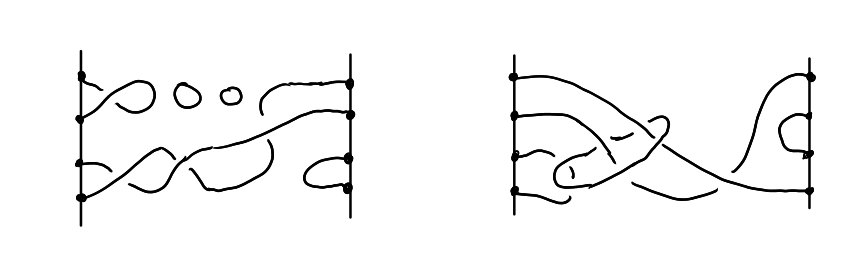
\includegraphics[scale=.25]{images/8.png}
\end{center}

\begin{remark}
\label{sec:temp-lieb-algebra}
  Any tangle diagram defined in this way (that is, the endpoints of strings on sides) can be turned into the general tangle diagram where the endpoints are on a circle. To see this, we simply connect the sides and expand it into a circle.
\end{remark}

Let $\Uplambda = \Z[A, A^{-1}]$ be the ring of Laurent polynomials and $\text{TA}_n(\delta)$ be a $\Uplambda$-algebra generated by $e_i$ for $1 \leq i \leq n$ satisfying the following relations 
\begin{align}
\label{eq:3}
\begin{split} 
  e_i^2 &= \delta e_i \\
  e_ie_{i\pm 1}e_i &= e_i \\
  e_ie_j &= e_je_i \hspace*{2em} \text{for } |i-j| > 1.
\end{split}
\end{align}
The $\Uplambda$-alegbra $\text{TL}_n(\delta)$ is called a Temperley-Leib algebra.

\begin{definition}
\label{sec:temp-lieb-algebra-1}
Let $R$ be a commutative ring and $\{ \gamma_n : B_n \to R \}_{n\geq 2}$ a sequence of functions such that the following conditions are satisfied.
\begin{enumerate}
\item\label{item:1} For two equivalent braids $\alpha, \beta \in B_n$ (equivalence under braid relations and isotopy), $\gamma_n(\alpha) = \gamma_n(\beta)$; 
\item\label{item:2} If $\alpha, \beta \in B_n$, then $\gamma_n(\beta) = \gamma_n(\alpha\beta\alpha^{-1})$ or equivalently, $\gamma_n(\alpha\beta) = \gamma_n(\beta\alpha)$;
\item\label{item:3} If $\beta \in B_n$, then there is a constant $a\in R$, independent of $n$, such that 
\begin{align}
\label{eq:5}
  \begin{split}
    \gamma_{n+1}(b\sigma_n) &= a \gamma_n(b) \\
    \gamma_{n+1}(b\sigma_n^{-1}) &= a^{-1} \gamma_n(b).
  \end{split}
\end{align}
\end{enumerate}
Then the sequence $\{\gamma_n\}$ is called a Markov trace on $\{B_n\}$.
\end{definition}

Let $\beta = \sigma_{i_1}^{r_{i_1}}\cdots\sigma_{i_k}^{r_{i_k}}$ be a braid in $B_n$. The writhe of $\beta$, denoted by $w(\beta)$, is defined to be the sum of the exponents $r_{i_1}, \ldots, r_{i_k}$. The Markov trace $\gamma_n\}$ can be used to construct invariants for links. Indeed, compare this with the Markov function we defined above.

\begin{theorem}
\label{sec:temp-lieb-algebra-2}
Let $\{ \gamma_n  \}$ be a Markov trace on $B_n$. Let $L$ be a link isotopic to a closed braid $\overline{\beta}$ (Alexander's theorem assures this). Set $\hat{\gamma}(L) = a^{-w(\beta)} \gamma_n(\beta) $. Then $\hat{\gamma}$ is an invariant for links.
\end{theorem}

The proof is quite similar to the one we wrote in the case of Markov functions. Observe that $w(\beta)$ is invariant under conjugation and braid isotopy and is used to cancel the effect of the second Markov move: $\beta \to \beta\sigma_n^{\pm 1}$.

Define $\left< \cdot \right> : B_n \to \Z[A, A^{-1}]$ such that the evaluation of $\left< \beta \right>$ is done on $\overline{\beta}$, the closed braid. By Alexander's theorem, we may reduce any given link $L$ to an isotopic closed braid $\overline{\beta}$. Given a closed braid $\overline{\beta}$, we may resolve all the crossings using the following skein relation.

\begin{align}
\label{eq:6}
\begin{split}
  \left<\KPB\right> &= A \left<\KPC\right> + A^{-1} \left<\KPD\right> \\
  \overline{\alpha} \coprod \KPA &= (-A^2 - A^{-2}) \overline{\beta}
\end{split}
\end{align}

A tangle is said be to reduced if there are no crossings and no additional loops. Indeed, using the skein relation given above any tangle can be reduced (if it is not already). Let $U_i$ for $1 \leq i \leq n-1$ be the tangles described below. See that they are tangles (just rotated by a right angle).
\vspace*{-.25em}
\begin{figure}[h]
  \centering
  \includegraphics[scale=.3]{images/tanglegenerators.png}
\end{figure}
\vspace*{-.25em}
Indeed, these $U_i$ are the generators all of reduced tangles, for one may write any reduced tangle as a composition of these $U_i$. Note that we are drawing the tangles in a special way (in a way very similar to geometric braid diagrams). The following relations are the abstraction of the isotopy of tangles.
\vspace*{-.25em}
\begin{figure}[h]
  \centering
  \includegraphics[scale=.3]{images/tanglerelations.png}
\end{figure}
\vspace*{-.25em}

The bracket $\left< \cdot \right>$ is defined for braids and tangles (later, we will see the same bracket extended to links). See that $\left< \sigma_i \right> = A\left< 1_n \right> + A^{-1}\left< U_i\right>$ where $1_n$ is the tangle with $n$ parallel strands. Similarly $\left< \sigma_i^{-1} \right> = A^{-1}\left< 1_n \right> + A\left< U_i \right>$ from the skein relation. We may omit $1_n$ and write $A\left< 1_n \right> + A^{-1}\left< U_i\right>$ as $A + A^{-1}\left< U_i\right>$.

  Let $A_n$ be an algebra over the ring $\mathbb{Z}[A, A^{-1}]$ of Laurent polynomials generated by the generators $U_i$ for $i = 1,\ldots, n-1$ and the following relations hold: 
\begin{align*}
  U_i^2 &= (-A^2-A^{-2}) U_i, \\
  U_iU_{i\pm 1}U_i &= U_i, \\
  U_iU_j &= U_jU_i, \hspace*{.6em} \text{if } |i-j|>1.
\end{align*}

See that $A_n$ is then the Temperley-Leib algebra $\text{TA}_{n-1}(-A^2-A^{-2})$. Suppose $U$ is a reduced tangle. If we take the closure of $U$, we get an unlink of trivial crossing-less components. Let $\sharp U$ be the number of components in this unlink minus $1$.

\begin{proposition}
\label{sec:temp-lieb-algebra-3}
The set $\{A + A^{-1}\left< U_i\right>\}$ for all $1 \leq i \leq n-1$ satisfy the braid relations.
\end{proposition}

Define a morphism $\rho_n : B_n \to A_n$ by 
\begin{align*}
  \sigma_i &\rightsquigarrow A + A^{-1}U_i, \\
  \sigma^{-1}_i &\rightsquigarrow A^{-1} + AU_i.
\end{align*}

The above proposition is equivalent to the following one.

\begin{proposition}
The map $\rho_n: B_n \to A_n$ is a representation of the braid group $B_n$.
\end{proposition}
\begin{proof}
It is easily checked that $\rho_n$ preserves the braid relations. That is, 
\begin{align*}
  \rho_n(\sigma_i)\rho_n(\sigma^{-1}_n) &= 1, \\
  \rho_n(\sigma_i\sigma_{i+1}\sigma_i) &= \rho_n(\sigma_{i+1}\sigma_i\sigma_{i+1}), \\
  \rho_n(\sigma_i\sigma_j) &= \rho_n(\sigma_j\sigma_i) \text{ if } |i-j|>1.
\end{align*}
Indeed, 
\begin{align*}
  \rho_n(\sigma_i)\rho_n(\sigma_i^{-1}) &= (A+A^{-1}U_i)(A^{-1} + AU_i) \\
                                        &= 1 + (A^{-2} + A^2)U_i + U_i^2 \\
                                        &= 1 + (A^{-2} + A^2)U_i + \delta U_i \\
                                        &= 1 + (A^{-2} + A^2)U_i + (-A^{-2} - A^2)U_i \\
  &= 1,
\end{align*}
\begin{align*}
  \rho_n(\sigma_i\sigma_{i+1}\sigma_i) &= (A+A^{-1}U_i)(A + A^{-1}U_{i+1})(A + A^{-1}U_i) \\
                                       &= (A^2 + U_{i+1} + U_i + A^{-2}U_iU_{i+1})(A + A^{-1}U_i) \\
                                       &= A^3 + AU_{i+1} + AU_i + A^{-1}U_iU_{i+1} + A^{-1}U_i^2 + AU_i + A^{-1}U_{i+1}U_i + A^{-3}U_iU_{i+1}U_i \\
                                       &= A^3 + AU_{i+1} + (A^{-1}\delta + 2A)U_i + A^{-1}(U_iU_{i+1} + U_{i+1}U_i) + A^{-3}U_i \\
                                       &= A^3 + AU_{i+1} + (A^{-1}(-A^2 - A^{-2}) + 2A + A^{-3})U_i + A^{-1}(U_iU_{i+1} + U_{i+1}U_i) \\
  &= A^3 + A(U_{i+1} + U_i) + A^{-1}(U_iU_{i+1} + U_{i+1}U_i),
\end{align*}
and as we can see, the final equation is symmetric in $i$ and $i+1$, and finally 
\begin{align*}
  \rho_n(\sigma_i\sigma_j) &= \rho_n(\sigma_i)\rho_n(\sigma_{j}) \\
                           &= (A+A^{-1}U_i)(A + A^{-1}U_j) \\
                           &= (A + A^{-1}U_j)(A + A^{-1}U_i) \\
  &= \rho_n(\sigma_j\sigma_i).
\end{align*}
This completes our proof that $\rho_n$ is a representation of the braid group.
\end{proof}

\begin{remark}
\label{sec:temp-lieb-algebra-4}
In the discussion above, the Temperley-Leib algebra $A_n$ was regarded as a $\Uplambda$-module. When we built the homomorphism $\rho_n: B_n \to A_n$, we regarded $A_n$ as a group under multiplication.
\end{remark}


The bracket polynomial (first introduced by Kauffman) is defined for knots and links using the same skein relation. Although it is not a link invariant (it fails to be invariant under the $\mathcal{R}^1$), we can normalize it so that it yields the famous Jones polynomial.

We shall now derive the bracket polynomial from our representation $\rho_n$ of the braid group. Let $\beta = \sigma^{a_1}_{i_1}\cdots \sigma^{a_k}_{i_k} \in B_n$ be some braid. Then
\begin{equation}
\rho_n(\beta) = \prod^k_{t=1} (A+A^{-1}U_{i_t})^{a_t} = \sum_s \langle \beta | s \rangle U_s,
\end{equation}
where $\langle \beta | s \rangle \in \mathbb{Z}[A, A^{-1}]$ is the coefficient of $U_s$ in the expansion of $\rho_n(\beta)$.

Define $\langle U_s \rangle = \delta^{\sharp U_s}$ and the bracket for the closed braid $\bar{\beta}$ by 
\begin{equation}
\langle \bar{\beta} \rangle = \sum_s \langle \beta | t \rangle \delta^{\sharp U_s}.
\end{equation}
Thus We have constructed a polynomial function for closed braids. This is the Kauffman bracket polynomial. As we can check, it fails to be invariant under Markov moves.

The bracket of the braid may be normalized as
\begin{equation}
  \langle \bar{\beta} \rangle = (-A^3)^{-w(\beta)} \sum_s \langle \beta | t \rangle \delta^{\sharp U_s}.
\end{equation}
  Given an oriented link $L$ in $\mathbb{R}^3$ we define 
\begin{equation}
V(L) = \langle \bar{\beta} \rangle,
\end{equation}
where $\beta$ is a braid whose closure is isotopic to $L$.

\begin{theorem}
The polynomial $V$ is a link invariant.
\end{theorem}
  
\begin{proof}
  Let $L$ and $L^{\prime}$ be two ambient isotopic links in $\R^3$. By Alexander's theorem, we can find two braids, $\beta$ and $\beta^{\prime}$ such that $L$ (resp. $L^{\prime}$) is isotopic to the closure of $\beta$ (resp. $\beta^{\prime}$). By Markov's theorem, $\bar{\beta}$ and $\overline{\beta^{\prime}}$ are related by a sequence of Markov moves. Therefore, it suffices to show that the normalized bracket $\langle \bar{\beta} \rangle$ is invariant under Markov moves. 
\begin{enumerate}
\item\label{item:8} For conjugation, we must check that $\langle \bar{\beta} \rangle = \left< \overline{\alpha\beta\alpha^{-1}} \right>$ for some $\alpha \in B_n$. It suffices to check that $\rho_n(\beta) = \rho_n(\alpha\beta\alpha^{-1})$. Since $\rho$ is a homomorphism, it suffices to check that $\rho_n(\beta) = \rho_n(\sigma_i\beta\sigma^{-1}_i)$. This can be checked by expansion: 
\begin{align*}
  \rho_n (\sigma_i\beta\sigma_i^{-1}) &= (A+A^{-1}U_i)\rho_n(\beta)(A^{-1} + AU_i) \\
                                      &= (A\rho_n(\beta) + A^{-1}U_i\rho_n(\beta) )(A^{-1} + AU_i) \\
                                      &= \rho_n(\beta) + (A^{-2} + A^2)U_i\rho_n(\beta) + U_i^2\rho_n(\beta) \\
                                      &= \rho_n(\beta) + (A^{-2} + A^2)U_i\rho_n(\beta) + (-A^{-2} - A^2)U_i\rho_n(\beta) \\
  &= \rho_n(\beta).
\end{align*}
\item\label{item:9} To show that the normalized bracket is invariant under $\beta \to \beta \sigma_n$, we first observe that $w(\beta \sigma_n) = w(\beta) + 1$. Then 
\begin{align*}
  \langle \overline{\beta\sigma_n}\rangle &= (-A^3)^{w(\beta) + 1} (\sum_t^{} \langle \beta | t \rangle \delta^{||U||})(A + A^{-1}\langle U_i \rangle) \\
                                          &= \langle \bar{\beta} \rangle (-A^3(A + A^{-1}\langle U_n \rangle)) \\
                                          &= \langle \bar{\beta} \rangle (-A^4 - A^2\langle U_n \rangle) \\
                                          &= \langle \bar{\beta} \rangle (-A^4 - A^2(-A^2 - A^{-2})) \\
                                          &= \langle \bar{\beta} \rangle (-A^4 + 1 + A^4) \\
  &= \langle \overline{\beta}\rangle.
\end{align*}
\item\label{item:7} Since $\rho_n$ is a braid representation, the possibility of equivalence in the braid group is also checked.
\end{enumerate}
This completes our proof that $V$ is an invariant for oriented links.
\end{proof}
 
\chapter{The Jones polynomial}
\label{chapter3}

The Jones polynomial $V_L(t^{1/2})$ is a function from the set of oriented links to the ring $\Z[t^{1/2}, t^{-1/2}]$ of Laurent polynomials. Sometimes by abuse of notation we will write $V_L(t)$ instead of $V_L(t^{1/2})$ as a shorthand for $t = (t^{1/2})^2$. Keeping in mind that the Jones polynomial is defined for oriented links $L$, we use the notations $V_L(t), V_L, V(L)$ to mean the same thing.

One characterizes $V_L(t)$ by giving the value $1$ to any diagram of the unknot (including the unknot diagrams with crossings) and satisfying the skein relation:
\begin{equation}
\label{2:eq:1}
  t^{-1}V_{L_+}(t) - tV(L_-) = (t^{1/2} - t^{-1/2})V(L_0),
\end{equation}
where $L_+$, $L_-$ and $L_0$ are oriented links that differ only locally as shown in the following diagram:

\begin{figure}[h]
  \centering
  \includegraphics[scale=.04]{images/jones-skein-relation.png}
\end{figure}
 
In some sources one finds the Jones polynomial defined in variable $t^{1/4}$. This is not necessary since it never really takes odd powers of $t^{1/4}$. Thus we have defined $V_L$ in variable $t^{1/2}$.

\begin{theorem}
\label{cha:jones-polynomial}
  The Jones polynomial $V_L(t)$ is an invariant for oriented links.
\end{theorem}

One may attempt to prove the above theorem using invariance under $\mathcal{R}^{1,2,3}$. We can also start with the definition Kauffman bracket and obtain the above skein relation. 

\begin{remark}
\label{cha:jones-polynomial-1}
  Suppose we compute $V_L(t)$ for $L_+$. By the above skein relation, we replace $V(L_+)$ by $V(L_-)$ and $V(L_0)$. Thus we are not strictly reducing to lower number of crossings since $V(L_+)$ and $V(L_-)$ has the same number of crossings.
\end{remark}

Although the above skein relation works well for computational purposes, we will use a different skein relation for the rest of our study. Let $L$ be an link. We compute $\langle L \rangle$ using the skein relation:
\begin{align*}
  \left< \KPA \right> &= -A^2 - A^{-2}, \\
  \left< \KPA D \right> &= (-A^2 - A^{-2}) \left< D \right>, \\
  \left< \KPB \right> &= A\left< \KPC \right> + A^{-1}\left< \KPD \right>.
\end{align*}
This polynomial $\left< \cdot \right>$ is called Kauffman bracket polynomial. Recall that we arrived at the bracket polynomial using Temperley-Lieb algebra in the previous chapter. 

\begin{remark}
\label{cha:jones-polynomial-2}
  Comparing the bracket skein relation with the skein relation we used above for $V_L(t)$, we see that while $V_L(t)$ needs orientation the bracket is defined without it.
\end{remark}

\begin{remark}
  Henceforth we will use the notations $L$ and $D$ interchangeably keeping in mind that $D$ is projection of $L$ onto the plane. The author prefers using $D$ and working with planar projections but the Jones polynomial $V_L(t)$ is written using $L$ in most literature.
\end{remark}

\begin{proposition}
\label{cha:jones-polynomial-3}
  The bracket polynomial $\left< \cdot \right>$ is characterized by the three bracket skein relations and invariance under $\mathcal{R}^2$ and $\mathcal{R}^3$.
\end{proposition}

Indeed, one may write down a general skein relation as the following:
\begin{align*}
  \left< \KPA \right> = \delta, \left< \KPA D \right> = \delta \left< D \right>, \left< \KPB \right> = A\left< \KPC \right> + B\left< \KPD \right>.
\end{align*}

The standard unknot (with no crossing) is associated with the value $\delta$. Our desire to make $\left< \cdot \right>$ invariant under $\mathcal{R}^2$ and $\mathcal{R}^3$ forces $B = A^{-1}$.

For an oriented link diagram, its crossing has a sign. A positive crossing $(+1)$ is the one associated with that crossing $L_+$ (in the skein relation above). Then a negative crossing $(-1)$ is the one associated with $L_-$ in that diagram. The writhe of the oriented link diagram, denoted by $w(D)$, is sum of the signs of all its crossings.

\begin{remark}
\label{cha:jones-polynomial-4}
  Adding or removing a kink ($\mathcal{R}^1$) changes the bracket by a factor of $-A^{\pm 3}$. This move also changes the writhe by $\pm 1$.
\end{remark}

\begin{theorem}
\label{cha:jones-polynomial-5}
The polynomial $p(D,A) = (-A)^{-3w(D)}\left< D \right>$ is an oriented link invariant.
\end{theorem}

By the above remark, the truth of the above theorem is easily established. Indeed one gets $V_L(t)$ from $p_D(A)$ by putting $A = t^{-1/4}$. This model of the Jones polynomial using the bracket has some advantages which we will utilize in the pages that follow. 

\begin{remark}
\label{cha:jones-polynomial-6}
  Since $V_L(t)$ has only powers of $t^{\pm 1/2}$, it follows that $p(D,A)$ has only powers of $A^{\pm 2}$.
\end{remark}

Let $D$ be an oriented link diagram. Using the bracket skein relation, we resolve all the crossings one by one. Each crossing can be resolved in two ways, one that gets multiplied by $A$ in the skein relation (we call this $A$-smoothing or $A$-splitting) and other one that gets multiplied by $A^{-1}$ (we call this $B$-smoothing or $B$-splitting). A glance at the general skein relation reveals why we have chosen to call it $B$-smoothing rather than $A^{-1}$-smoothing.

A state $S$ is a map from the set of crossings of $D$ to the set $\{A, B\}$. If $D$ has $n$ crossings, then there are $2^n$ states. These are all the possible ways to resolve the crossings. Let $\mathcal{S}(D)$ denote the set of all states (later, we will turn $\mathcal{S}(D)$ into a category). For a state $S$, denote by $a(S)$ and $b(S)$, the number of $A$-smoothings and $B$-smoothings respectively in $S$. Put $\sigma(S) = a(S) - b(S)$. Once we resolve all the crossings, we end up with a bunch of topological circles. For a state $S$, we denote the number of circles by $\sharp S$.

\begin{theorem}
\label{cha:jones-polynomial-7}
  The bracket polynomial can be written as the following sum: 
\begin{equation}
\label{2:eq:2}
\left< D \right> = \sum_{S\in\mathcal{S}(D)}^{}  A^{\sigma(S)}(-A^2 - A^{-2})^{\sharp S - 1}.
\end{equation}
\end{theorem}

This theorem follows from the bracket skein relations. A state $S$ has $\sharp S$ circles, hence $\left< S \right> = (-A^2 - A^{-2})^{\sharp S - 1}$. Each $A$-smoothing gets multiplied by $A$ and each $B$-smoothing gets multiplied by $A^{-1}$. Thus each state $S$ contributes $A^{\sigma(S)}(-A^2 - A^{-2})$ to the sum where $\sigma = a(S) - b(S)$. This proves the theorem.

Let us call this the state-sum model of $\left< \cdot \right>$. We will make great use of it in proving propositions and theorems. See that the Jones polynomial $p(D,A)$ also admits a similar state-sum model. We list this result as a theorem due to its importance in the work that will follow.

\begin{theorem}
\label{cha:jones-polynomial-8}
The Jones polynomial $p(D, A)$ can be written as the following sum: 
\begin{equation}
\label{eq:1}
p(D,A) = (-1)^{-3w(D)} \sum_{S\in \mathcal{S}(D)}^{} A^{\sigma(S) - 3w(D)} (-A^2 - A^{-2})^{\sharp S - 1}.
\end{equation}
\end{theorem}

In our definition, we have normalized $\left< \KPA \right> = 1$. By applying the second skein relation, we must have $\left< \emptyset \right> = 1/(-A^2-A^{-2})$ for the empty link $\emptyset$. This is not a Laurent polynomial and does not look elegant. Thus we may normalize $\left< \KPA \right> = -A^2 - A^{-2}$ so that $\left< \emptyset \right> = 1$. We make no changes to the second and third skein relation. Thus the normalization preserves its invariance under $\mathcal{R}^2$ and $\mathcal{R}^3$. We will call this unreduced bracket polynomial and denote it by $\left< \hat{\cdot} \right>$. The same normalization applied to the Jones polynomial yields the unreduced Jones polynomial denoted by $\hat{p}(L,A)$.

One may normalize by giving $\left< \KPA \right>$ other values. One can introduce variable changes as well. For instance, substituting $A = t^{-1/4}$ in $p(L,A)$ yielded $V_L(t)$. Later when we study Khovanov homology we will substitute $q = -A^{-2}$ and work with $\hat{J}_L(q)$. Indeed one uses different normalizations and variable changes for different purposes and it may become difficult to know which one is which. For our work, we will use $\hat{J}_L(q)$ (introduced later) for Khovanov homology, $p(L,A)$ when we want to exploit the state-sum model (starting next chapter) and $V_L(t)$ for other purposes.

For an oriented link $L$, one obtains its mirror-image, denoted by $\overline{L}$, by applying $\KPB \to \KPE$ or $\KPE \to \KPB$ (whichever applicable) to each of the crossings. A link is said to be \emph{amphicheiral} (or \emph{acheiral}) if it is ambient isotopic to its mirror image. A chiral link is one which is not amphicheiral. The simplest chiral knot is the trefoil since $3_1$ and $3_2$ are mirror images and $3_1 \ncong 3_2$. The Jones polynomial is useful in detecting chirality.

\begin{theorem}
\label{cha:jones-polynomial-9}
  Let $L$ be an oriented link and $\overline{L}$ its mirror-image. Then 
\begin{equation}
\label{eq:2}
V_{\overline{L}}(t) = V_L(t^{-1}), \ p(\overline{D}, A) = p(D, A^{-1}).
\end{equation}
\end{theorem}

\begin{proof}
  Since the two equations are equivalent, we will establish only $p(\overline{D}, A) = p(D, A^{-1})$. In taking mirror-image, we apply $\KPB \to \KPE$ or $\KPE \to \KPB$. This reverses the sign of all the crossings. Thus $w(\overline{D}) = -w(D)$. From the skein relation $\left< \KPB \right> = A\left< \KPC \right> + A^{-1}\left< \KPD \right>$, one sees that the bracket $\left< \overline{D} \right>$ is just $\left< D \right>$ with $A$ and $A^{-1}$ exchanged. By Theorem \ref{cha:jones-polynomial-5}, it follows that $p(\overline{D}, A) = p(D, A^{-1})$.
\end{proof}

\begin{corollary}
\label{cha:jones-polynomial-10}
  Let $K$ be a knot. If the Jones polynomial $V_K(t)$ is not symmetrical under the exchange $t \leftrightarrow t^{-1}$ or equivalently, $V_K(t) \ne V_K(t^{-1})$, then $K$ is chiral.
\end{corollary}

The truth is obvious since $V_K(t)$ is an invariant. Thus we have found the first major use of $V_L(t)$. One may quickly verify that $V_{3_1}(t) \ne V_{3_1}(t^{-1})$.

\begin{remark}
\label{cha:jones-polynomial-11}
The converse of the above corollary is not true and hence this method cannot detect all the chiral knots. There exist chiral knots $K$ with $V_K(t) = V_K(t^{-1})$.
\end{remark}

Note that not all polynomial invariants can detect chirality. The Alexander polynomial cannot detect chirality.

\begin{remark}
\label{cha:jones-polynomial-12}
In Theorem \ref{cha:jones-polynomial-9}, we considered oriented link $L$ while in Corollary \ref{cha:jones-polynomial-10}, we considered knot $K$. The reason will become evident from the next few results. 
\end{remark}

\begin{proposition}
  \label{cha:jones-polynomial-13}
  The Jones polynomial $V_K(t)$ of a knot $K$ is independent of orientation.
\end{proposition}

\begin{proof}
\label{cha:jones-polynomial-14}
By the Jones skein relation ($\ref{2:eq:1}$), reversing the orientation of a knot leaves $L_+$ and $L_-$ unchanged (signs of crossings are preserved). The result follows.
\end{proof}

\begin{remark}
\label{cha:jones-polynomial-15}
By the same logic, reversing the orientation of all the components of a link $L$ also leaves $V_L(t)$ unchanged.
\end{remark}

In general, changing orientation of some (but not all) components of a link $L$ may change $V_L(t)$. A simple example is the Hopf link. In the following is a brilliant result that says that changing orientation of some components of a link multiplies $V_L(t)$ by some power of $t$. Before that we need a definition. Let $L$ be an oriented $n$-component link with components labelled $L^i$ for $1 \leq i \leq n$. The linking number $lk(L^i, L^j)$ is half of the sum of signs of crossings where a segment of $L^i$ crosses $L^j$. These signs ($+1$ or $-1$) follow the same convention as the writhe. Given an oriented link diagram with $n$ components, there are such $\binom{n}{2}$ linking numbers corresponding to each pair of components.

\begin{proposition}
\label{cha:jones-polynomial-16}
The linking number is an invariant.
\end{proposition}

\begin{proof}
The move $\mathcal{R}^1$ affects only one component of a diagram and can, thus, be ruled out. The move $\mathcal{R}^2$ introduces or deletes two crossings with opposite sign which does not affect $lk(L^i, L^j)$. Similarly $\mathcal{R}^3$ also leaves $lk(L^i, L^j)$ unchanged.
\end{proof}

For a link $L$, we write $L = \coprod^n L^i$ to specify that $L$ is an $n$-component link with each component labelled $L^i$. We may write simply $L = \coprod L^i$ if $n$ is unimportant or unknown. For greater generality, we extend this notation and write $L = M\coprod N$ where $M$ and $N$ are possibly links themselves. We write $rN$ to denote the same link $N$ but orientation of each component reversed.

We extend the definition of linking number as well. For oriented links $M$ and $N$, define $lk(M,N) = \sum_{i,j}^{} lk(M^i, N^j)$, where the sum is over all possible pairs of components of $M$ and $N$.

\begin{theorem}
\label{cha:jones-polynomial-17}
Let $L = M \coprod N$ be an oriented link. Let $L^{\prime} = M \coprod rN$ be the link obtained by reversing the orientation of all the components of $N$. Let $\lambda = lk(M,N)$. Then
\begin{equation}
\label{eq:3}
V_{L^{\prime}}(t) = t^{-3\lambda}V_L(t).
\end{equation}
\end{theorem}

\begin{proof}
  Recall that $V_L(t) = p(L,A) = (-A)^{-3w(L)}\left< L \right>$ and $\left< \cdot \right>$ is invariant under $\mathcal{R}^2$ and $\mathcal{R}^3$. Clearly $\left< L \right>$ is unaffected by change in orientation in any number of components of $L$. Thus only the writhe is changed. See that changes in crossing sign happen only at the sites where some $M^i$ meets some $N^i$. Observe that $lk(M,N)$ involves the same crossings. We denote a crossing between $M^i$ and $N^i$ by $x(M^i,N^j)$. We denote its sign by sgn$(x(M^i,N^j))$. Since writhe decreases by $2$ when a positive crossing changes to a negative crossing and increases by $2$ when a negative crossing changes to a positive, it follows that 
\begin{equation}
w(L^{\prime}) = w(L) - 2 \sum_{i,j,x}^{}\text{sgn} (x(M_i,N_j)) = w(L) - 4lk(M,N).
\end{equation}
From the above equation, it follows that 
\begin{equation}
\label{eq:4}
(-A)^{-3w(L)} = (-A)^{-3w(L^{\prime})}(-A)^{-12\cdot lk(M,N)}.
\end{equation}
Substituting $A^{-4} = t$ and $\lambda = lk(M,N)$, we have $V_{L^{\prime}}(t) = t^{-3\lambda} V_L(t)$.
\end{proof}

Notwithstanding that $V_L(t)$ depends on the orientation of some of the components of $L$, Theorem \ref{cha:jones-polynomial-17} equips us with a tool to control this dependence. Indeed, one may define a variant of the Jones polynomial which does not depend on the orientation. The construction is obvious and straightforward.

Define self-writhe of a link $L$ as $\hat{w}(L) = w(L) - 2 \sum_{i,j}^{}lk(L^i,L^j)$. Alternatively, $\hat{w}(L) = \sum_i^{}w(K^i)$, where $K^i$ is $L^i$ considered as a knot (that is, ignoring every other component $L^j$ where $i \ne j$). Obviously $\hat{w}(L)$ is $\mathcal{R}^{2,3}$-invariant and gets multiplied by $A^{\pm 1}$ under $\mathcal{R}^1$ in the way $w(L)$. Clearly $\hat{w}(D)$ is independent of orientation (by the same argument used in the proof of Proposition \ref{cha:jones-polynomial-13}). Define $f(L, A) = (-A)^{-3\hat{w}(L)}\left< L \right>$ and then put $A = t^{-1/4}$ to define $V^{\prime}_L(t)$. The Jones polynomial $V^{\prime}_L(t)$ is then defined and is an invariant for unoriented links.

There are two two-variable polynomial invariants that generalize $V_L(t)$. They are the HOMFLY (or HOMFLYPT) polynomial and the Kauffman polynomial. The HOMFLY polynomial is defined (indeed, well-defined) by the following theorem.

\begin{theodef}
\label{cha:jones-polynomial-19}
There exists a unique map $P$ from $\mathcal{L}/(\cong)$, the set of oriented links under equivalence of ambient isotopy, to $\Z[l^{\pm}, m^{\pm}]$ such that $P(\KPA) = 0$ and 
\begin{equation}
\label{eq:5}
lP(L_+) + l^{-1}P(L_-) + mP(L_0) = 0,
\end{equation}
where $L_+, L_-$ and $L_0$ differ only locally at the points indicated below.
\begin{figure}[h]
  \centering
  \includegraphics[scale=.04]{images/jones-skein-relation.png}
\end{figure}
\end{theodef}
The polynomial $P$ is called the HOMFLY polynomial. The proof for existence and uniqueness relies on induction on the number of crossings \cite{lickorish1997}. The HOMPLY polynomial may well be regarded as polynomial in three variables $x,y,z$ hence belonging to the ring $\Z[x^{\pm}, y^{\pm}, z^{\pm}]$ with the skein relation $xP(L_+) + yP(L_-) + zP(L_0) = 0$.

\begin{remark}
The condition $P(\KPA) = 0$ applies to all knots isotopic to $\KPA$. Indeed, this is already implied in the definition since the domain of $P$ is $\mathcal{L}/(\cong)$.
\end{remark}

\begin{theorem}
\label{cha:jones-polynomial-18}
There exists a unique map $\Theta$ from the set of unoriented links to $\Z[a^{\pm}, z^{\pm}]$ such that 
\begin{enumerate}[font=\upshape]
\item\label{item:1} Normalization: $\Theta(\KPA) = 0$ (the crossing-less unknot);
\item\label{item:2} Invariance: $\Theta(\cdot)$ is $\mathcal{R}^{2,3}$-invariant; 
\item\label{item:3} Effect under $\mathcal{R}^1$: $\Theta(s_r) = a\Theta(s)$, $\Theta(s_l) = a^{-1}\Theta(s)$; 
\item\label{item:4} Skein relation: 
\begin{equation}
\label{3:eq:6}
\Theta(\KPB) + \Theta(\KPE) = z\Theta(\KPC) + z\Theta(\KPD),
\end{equation}
\end{enumerate}
where $s$ is an arc and $s_r$ (resp. $s_l$) is the same arc with a right-handed (resp. left-handed) curl added ($\mathcal{R}^1$).
\end{theorem}

\begin{definition}
\label{cha:jones-polynomial-21}
The Kauffman polynomial is a map from the set of unoriented links to $\Z[a^{\pm}, z^{\pm}]$ defined by $K(L) = a^{-w(L)} \Theta (L)$, where $\hat{w}(L)$ is the self-writhe of $L$.
\end{definition}

\begin{remark}
The writhe $w(D)$ in the definition may be replaced by $\hat{w}(D)$ since both are $\mathcal{R}^{2,3}$-invariant and $a^{-w(L)} \Theta (L)$ is an invariant for unoriented links as well. Indeed, using $\hat{w}(L)$ would have been a better choice since it does not require computation of $lk(L^i,L^j)$ but the use of $w(L)$ is standard and well-established.
\end{remark}

The new polynomials $P(L)$ and $K(L)$ share several of the properties we derived for $V_L(t)$.

\begin{remark}
  As we have seen in this chapter and will see in the subsequent chapters, some problems are easier solved using $p(L,A)$ while others are easier with $V_L(t)$.
\end{remark}


% mutation effects
\chapter{Khovanov Homology}

\section{Introduction}

\section{The Cube Category}

\section{Categorification of the Jones Polynomial}

\section{}

\section{}

\section{}

\section{}

  
\chapter{Categorification}
\label{chapter5}

\section{Homology theories}

The Euler characteristic $\chi$ is a topological invariant. That is, two topological spaces belonging to the same homeomorphism class have the same $\chi$. For a polyhedron, it is given by $\chi = v - e + f$, where $v, e$ and $f$ are respectively the number of vertices, edges and faces. One may generalize this to a definition valid for simplicial complexes. A simplicial complex is a set composed of simplexes. A $0$-simplex is just a point, $1$-simplex is an edge, $2$-simplex is a triangle (consisting of its interior), $3$-simplex is a solid tetrahedron and $n$-simplex is a higher-dimensional analogue. One easily sees that the definition of $\chi$ valid for simplicial complexes should then be 
\begin{equation}
\label{eq:1}
\chi(X) = k_0 - k_1 + k_2 - k_3 + \cdots = \sum_{n=0}^{\infty} (-1)^n k_n, 
\end{equation}
where $k_n$ is the number of $n$-simplexes in $X$. Putting $k_0 = v$, $k_1 = e$, $k_2 = f$ and $k_n = 0$ for higher $n$ reduces this definition to the polyhedron case. Still more generally, we may define free abelian groups $C_n(X)$ so that $\chi$ appears as an alternating sum of the ranks of these groups: 
\begin{equation}
\label{eq:2}
\chi(X) = \sum_n^{\infty} (-1)^n \text{ rk}C_n(X).
\end{equation}
One easily sees that $\text{rk } C_n(X) = k_n$ so that the definitions agree. Thus, $C_n$ must be free abelian groups generated by the $n$-simplexes.

The following chain of free abelian groups is commonly referred to as a chain complex.
\begin{equation}
\label{eq:3}
\cdots \to C^n \xrightarrow{\partial_n} C^{n-1} \xrightarrow{\partial_{n-1}} \cdots \xrightarrow{\partial_3} C_2 \xrightarrow{\partial_3} C_1 \xrightarrow{\partial_1} C_0 \to 0.
\end{equation}
In the above chain complex, all but finitely many $C_n$ are zero. Further, $\partial_n \partial_{n-1} = 0$ (commonly written as $\partial^2 = 0$), where the map $\partial$ (called the differential or boundary operator) maps simplexes to their boundaries. The condition $\partial^2 = 0$ (a necessary condition for chain complexes) is equivalent to saying that boundary of a boundary is zero (or rather, a boundary has no boundary). The homology groups $H_n(X)$ are defined as 
\begin{equation}
\label{eq:4}
H_n(X) = \frac{\ker \partial_n}{\text{im }\partial_{n-1}}.
\end{equation}

Further still, simplicial homology may be generalized to singular homology. We still have a similar looking chain complex with $\partial^2 = 0$ and the homology groups are defined in the same way. If the groups $H_n(X)$ have finite rank, it turns out that rk $(C_n) = $ rk $(H_n(X))$.

The homology groups $H_n(X)$ are more fundamental to the topological space $X$ than its Euler characteristic $\chi(X)$. Besides, $H_n$ is a functor from the category of chain complexes to the category of abelian groups.

Later, inspired by the homology theory for spaces, we will construct a homology theory for links such that the graded Euler characteristic of this homology turns out to be the Jones polynomial.

\section{Categories and functors}

Let $R$ be a commutative ring. Chain complexes of $R$-modules form a category $Kom_R$ (sometimes denoted by $Ch_R$ in some texts) in which objects are chain complexes $(C_{*},\partial_{*})$ and a morphism from a chain complex $(C_{*},\partial_{*})$ to another chain complex $(C^{\prime}_{*}, \partial^{\prime}_{*})$ is a sequence of homomorphisms $\psi_n : C_n \to C^{\prime}_n$ such that $\psi_{n-1} \circ \partial_n = \partial^{\prime}_n \circ \psi_n$ for all $n$. That is, the following diagram
\begin{equation}
\label{eq:6}
\begin{tikzcd} 
  \cdots \arrow[r, "\partial_{n+2}"] & C_{n+1} \arrow[r, "\partial_{n+1}"] \arrow[d, "\psi_{n+1}"] & C_n \arrow[r, "\partial_n"] \arrow[d, "\psi_n"] & C_{n-1} \arrow[d, "\psi_{n-1}"] \arrow[r, "\partial_{n-1}"] & \cdots\\
  \cdots \arrow[r, "\partial^{\prime}_{n+2}"] & C^{\prime}_{n+1} \arrow[r, "\partial^{\prime}_{n+1}"] &  C^{\prime}_{n} \arrow[r, "\partial^{\prime}_n"] & C^{\prime}_{n-1} \arrow[r, "\partial^{\prime}_{n-1}"] & \cdots
\end{tikzcd}
\end{equation}
commutes. As noted above, $H_n$ is a functor from $Kom_R$ to $R$-\textbf{Mod} (abelian groups are $\Z$-modules).

Let $X, Y$ be spaces and $f: X \to Y$ be a continuous map (hence a morphism in \textbf{Top}). Then $f$ induces a chain map or morphism $(C_{*}(X), \partial_{*}(X)) \to (C_{*}(Y), \partial_{*}(Y))$ in $Kom_R$. From the discussion above, it follows that $H_n$ is a functor from \textbf{Top} to $R$-\textbf{Mod}.

% \section{Categorification of the Jones polynomial}

\chapter{Khovanov homology}
\label{chapter6}

\section{Categorification of $\hat{J}_L(q)$}

The bracket polynomial may be normalized in the following way: 
\begin{align*}
  \left[ \KPA \right] &= q+q^{-1}, \\
  \left[ \KPA D \right] &= (q+q^{-1}) \left[ D \right], \\
  \left[ \KPB \right] &= \left[ \KPC \right] - q^{-1}\left[ \KPD \right].
\end{align*}

Observe that we used the symbol $[D]$ to denote the bracket polynomial defined in this way.
\begin{proposition}
\label{sec:cohom-groups-mathc-1}
The bracket $[D]$ is $\mathcal{R}^{2,3}$ but changes by a factor of $q^{\pm 1}$ or $-q^{\pm 2}$ under $\mathcal{R}^1$.
\end{proposition}

This is easily checked.

Let $n$ be the number of crossings in the link diagram $D$. Let $n_+$ and $n_-$ be the number of positive crossings and negative crossings in $D$ such that $w(D) = n_+ - n_-$. Define the unnormalized Jones polynomial as
\begin{equation}
\label{eq:3}
\hat{J}(D) = (-1)^{n_-} q^{n_+ - 2n_-} [D].
\end{equation}

\begin{theorem}
\label{sec:cohom-groups-mathc-4}
The polynomial $\hat{J}(D)$ is an invariant for oriented links. The usual Jones polynomial $J(D)$ is related to $\hat{J}(D)$ by the relation 
\begin{equation}
\label{eq:4}
J(D) = \hat{J}(D)/(q + q^{-1}).
\end{equation}
\end{theorem}

\begin{proof}
\label{sec:cohom-groups-mathc-5}
The term $(-1)^{n_-} q^{n_+ - 2n_-}$ is $\mathcal{R}^{2,3}$-invariant. By Proposition \ref{sec:cohom-groups-mathc-1}, adding or removing a positive kink multiplies the bracket by a factor of $q^{\pm 1}$ and adding or removing a negative kink multiplies the bracket by a factor of $-q^{\pm 2}$. The term $(-1)^{n_-} q^{n_+ - 2n_-}$ negates the changes in bracket polynomial under $\mathcal{R}^1$. Since $\hat{J}(D)$ is normalized by giving the unknot a value of $q + q^{-1}$, we simply divide $\hat{J}(D)$ by this value to get the usual Jones polynomial $J(D)$.
\end{proof}
\begin{remark}
\label{sec:cohom-groups-mathc-7}
One may obtain the Jones polynomial $V_L(t)$ by substituting $q = -t^{1/2}$.
\end{remark}

Using the skein relation, each crossing of $D$ can be smoothed in two ways---$1$-smoothing (in which bracket polynomial gets multiplied by $q^{-1}$) and $0$-smoothing. Let $\sharp 1$ be the number of $1$-smoothings and $\sharp S$ the number of circles (loops) for a state $S$.

\begin{proposition}
\label{sec:cohom-groups-mathc-6}
Let $\mathcal{S}$ be the set of all states of an oriented link diagram $D$. Then the bracket $[D]$ can be written as a state-sum: 
\begin{equation}
\label{eq:5}
[D] = \sum_{S \in \mathcal{S}}^{} (-1)^{\sharp 1} q^{\sharp 1} (q + q^{-1})^{\sharp S}.
\end{equation}
\end{proposition}

\begin{proof}
\label{sec:cohom-groups-mathc-8}
Each state $S$ has $\sharp S$ circles and each circle has the bracket $q + q^{-1}$. Each time a crossing receives a $1$-smoothing, the bracket changes by a multiple of $-q$. Since state $S$ has $\sharp 1$ number of $1$-smoothings, it is easy to see that each contributes $(-1)^{\sharp 1} q^{\sharp 1} (q + q^{-1})^{\sharp S}$ to the sum. 
\end{proof}

\begin{theorem}
\label{sec:cohom-groups-mathc-9}
The unnormalized Jones polynomial $\hat{J}(D)$ can be written as a state-sum: 
\begin{equation}
\label{eq:6}
\hat{J}(D) = \sum_{S\in \mathcal{S}}^{} (-1)^{n_- + \sharp 1} q^{n_+ - 2n_- + \sharp 1} (q+q^{-1})^{\sharp S}.
\end{equation}
\end{theorem}

\begin{proof}
\label{sec:cohom-groups-mathc-10}
It follows trivially from the definition of $\hat{J}(D)$ and Proposition \ref{sec:cohom-groups-mathc-6}.
\end{proof}

Assign an arbitrary order of the crossings of $D$. A state $S$ may be represented by a binary sequence of length $n$. The bit $0$ or $1$ denote the type of smoothing for each crossing. That is, any state is of the form $x_1x_2\cdots x_n$ where $x_i = 0$ if the $i$th crossing has $0$-smoothing, otherwise $x_i = 1$. See that there is a one-to-one correspondence between the set $\mathcal{S}$ of states and the set of all binary sequences of length $n$.

The states in $\mathcal{S}$ form a category, denoted by $\mathcal{S}(D)$. The objects in $\mathcal{S}(D)$ are the states of $D$ (represented as binary sequences) while morphisms $S_1 \to S_2$ are such that $S_2$ is obtained from $S_1$ by changing a single $0$-smoothing in $S_1$ to $1$-smoothing. Speaking in terms of binary sequences, we have the morphism 
\begin{displaymath}
x_1\cdots x_i \cdots x_n \to x_1\cdots x_i^{\prime} \cdots x_n,
\end{displaymath}
where $x_i = 0$ and $x_i^{\prime} = 1$, and every other bit is left unchanged.

There is a notation for such a morphism. We use the asterisk $*$ to denote where the change of smoothing from $0$ to $1$ occurs. For instance,
\begin{displaymath}
000 \xrightarrow{0*0} 010 \xrightarrow{*10} 110 \xrightarrow{11*} 111.
\end{displaymath}
The state category $\mathcal{S}(D)$ can be given some extra structure. Each state object has a height $\sharp 1$ (the number of $1$-smoothings) associated with it. For instance, $0\cdots0$ is the only state with height $0$ and $1\cdots 1$ is the only state with height $n$. Every other state has a height between $0$ and $n$. All state objects can then be represented in a diagram according to their heights. All state objects with the same height are placed in the same column and the arrows go from left to right in the direction of increasing height. The following are state categories for the Hopf link and the trefoil.

\begin{figure}[h]
  \centering
  \includegraphics[scale=.35]{images/Hopfcat.png}
\end{figure}

\begin{figure}[h]
  \centering
  \includegraphics[scale=.35]{images/cubecat.png}
\end{figure}

A state diagram is simply a bunch of circles. Let $S_1 \to S_2$ be a morphism in the state category $\mathcal{S}(D)$. Now we see $S_i$ as a bunch of circles and not as a binary sequence. Observe that two things can happen here. Either two circles in $S_1$ fuse together to form a circle in $S_2$ or a circle in $S_1$ bifurcates into two circles $S_2$, while every other circle remain untouched. Observe that in each case $S_1 \to S_2$ can be thought of as a surface cobordism since a disjoint union of circles form a $1$-manifold. These cobordisms are directed down the page as shown below.

\begin{figure}[h]
  \centering
  \includegraphics[scale=.1]{images/cobordism.png}
\end{figure}

From the discussion above, we have another category whose objects are states seen as disjoint union of circles and whose morphisms are surface cobordisms. It is taken care that this morphism (surface cobordism) is one of the two types shown above. We denote this category by $Cob\mathcal{S}(D)$. See that $Cob\mathcal{S}(D)$ shares the same height structure we associated to $\mathcal{S}(D)$ although this has become less apparent. This can be seen from the equivalence of the categories $Cob\mathcal{S}(D)$ and $\mathcal{S}(D)$. An appropriate functor $\mathcal{S}(D) \to Cob\mathcal{S}(D)$ that builds this equivalence should assign to each object of $Cob\mathcal{S}(D)$ its correct height.

\begin{proposition}
\label{sec:cohom-groups-mathc-11}
Let $\mathcal{A}$ be a category. Let $Mat(\mathcal{A})$ be the set of all possible tuples of objects of $\mathcal{A}$. A morphism from a $p$-tuple $\mathcal{O} = (\mathcal{O}_1, \ldots, \mathcal{O}_p)$ to a $q$-tuple $\mathcal{O}^{\prime} = (\mathcal{O}_1^{\prime}, \ldots, \mathcal{O}_q^{\prime})$ is defined to be the matrix $[d_{ij}]_{p\times q}$ where $d_{ij}$ is the morphism $\mathcal{O}_i \to \mathcal{O}_j^{\prime}$. Then $Mat(\mathcal{A})$ forms a category in which objects are tuples of objects of $\mathcal{A}$ and morphisms are the matrices as defined above. The composition of morphisms is given by matrix multiplication.
\end{proposition}

The proof follows by construction. One simply checks that all requirements of a category are satisfied.

Look at $Mat(Cob\mathcal{S}(D))$. The category $Mat(Cob\mathcal{S}(D))$ is constructed from $Cob\mathcal{S}(D)$ in the way $Mat(\mathcal{A})$ is constructed from $\mathcal{A}$ in Proposition \ref{sec:cohom-groups-mathc-11}. Further, we ensure that the following two conditions are satisfied. 
\begin{enumerate}
\item\label{item:1} If there is no morphism (cobordism) $S_i \to S_j$ in $Cob\mathcal{S}(D)$, we equate $d_{ij} = 0$.
\item\label{item:2} Each object in $Mat(Cob\mathcal{S}(D))$ is of the form $\mathcal{O}^h = (S_1, \ldots, S_k)$ where each $S_i$ has height $h$ (that is, $\sharp 1 = h$) and these are all the states with height $h$.
\end{enumerate}

These two conditions ensure that we end up with something like the following: 
\begin{equation}
\label{eq:7}
\mathcal{O}^{0} \xrightarrow{d^0} \mathcal{O}^1 \xrightarrow{d^1} \mathcal{O}^2 \xrightarrow{d^2} \cdots \xrightarrow{d^{n-1}} \mathcal{O}^{n}.
\end{equation}

In the above, we have collapsed all states with the same number of $1$-smoothings into an object $\mathcal{O}^h$. For the sake of completion, we may add the initial object $\hat{0}$ and the final object $\hat{1}$ in $Mat(Cob\mathcal{S}(D))$. In fact, we can equate $\hat{0} = \hat{1}$ if we define both of them to be empty tuples. Then by this construction $Mat(Cob\mathcal{S}(D))$ becomes a pointed category (a pointed category is one with a zero element, that is, the initial object and final object exist and are isomorphic).
\begin{equation}
\label{eq:8}
\hat{0} \xrightarrow{0} \mathcal{O}^{0} \xrightarrow{d^0} \mathcal{O}^1 \xrightarrow{d^1} \mathcal{O}^2 \xrightarrow{d^2} \cdots \xrightarrow{d^{n-1}} \mathcal{O}^{n} \xrightarrow{0} \hat{0}.
\end{equation}

The morphism $0$ in the above category is zero map, that is, it satisfies $d^i \cdot 0 = 0 = 0\cdot d^i$.

This reminds us of a chain complex except that $\mathcal{O}^h$ are tuples of states and not abelian groups (or modules) and we have not established that $d^{i+1} \circ d^{i} = 0$. But both of these problems can be fixed and we can indeed have a chain complex this way. We shall come back to this later. Now we digress to something else.

A graded vector space is a decomposition of a vector space into a direct sum of subspaces. Let $W$ be a $\Z$-graded vector space. Then 
\begin{displaymath}
W = \bigoplus_{m\in\Z} W_m,
\end{displaymath}
where each $W_m$ is a subspace of $W$. The subspace $W_m$ is said to have degree $m$ and its elements are said to be homogeneous elements of degree $m$.

Although $\Z$ grading is used above, any indexing set $\mathcal{I}$ may also be used. We stick to $\Z$ grading. The graded dimension of $W$, denoted by $\dim_q W$, is defined to be the power series
\begin{equation}
\label{eq:9}
\dim_q W(q) \coloneqq \sum_{m \in \Z}^{} q^m \dim(W_m).
\end{equation}

\begin{proposition}
\label{sec:cohom-groups-mathc-12}
Let $W = \bigoplus_m W_m$ and $W^{\prime} = \bigoplus_m W_m^{\prime}$ be two $\Z$-graded vector spaces. Then 
\begin{align}
\label{eq:1}
  \dim_q (W \oplus W^{\prime}) &= \dim_q W + \dim_q W^{\prime}, \\
\label{eq:2}
  \dim_q (W \otimes W^{\prime}) &= \dim_q W \cdot \dim_q W^{\prime}.
\end{align}
\end{proposition}

The proof follows from the definition given by Equation \ref{eq:9} and expansion of the terms. 

\begin{proposition}
\label{sec:cohom-groups-mathc-13}
Given a $\Z$-graded vector space $W = \bigoplus_{m} W_m$, define shifting operation, denoted by $\{l\}$, by $W\{l\}_m \coloneqq W^{m-l}$ so that $W\{l\} = \bigoplus_m W\{l\}_m$. Then 
\begin{equation}
\label{eq:10}
\dim_qW\{l\} = q^l \dim_q W.
\end{equation}
\end{proposition}

Let $V = \F_2[x]/(x^2)$. We may also use $\Z$ or $\Q$ instead of $\F_2$. This algebraic structure can be viewed in different ways. First, $V$ can be realized as a graded vector space. A basis would be $\{1, x\}$. By grading  $\deg(1) = 1$ and $\deg(x) = -1$, it follows that $\dim_q V = q + q^{-1}$. This choice of grading is not random since the bracket polynomial has been normalized so that its value for the crossingless unknot is $q+q^{-1}$.

Consider the $k$th tensor product $V^{\otimes k}$. Then $\dim_q V^{\otimes k} = (q + q^{-1})^k$. By shifting $\{r\}$, it follows that $\dim_q V^{\otimes k}\{r\} = q^r (q + q^{-1})^k$. Substituting $r = n_+ - 2n_- + \sharp 1$ and $k = \sharp S$, it follows that 
\begin{equation}
\label{eq:11}
\dim_q V^{\otimes \sharp S} \{ n_+ - 2n_- + \sharp 1 \} = q^{n_+ - 2n_- + \sharp 1} (q + q^{-1})^{\sharp S}.
\end{equation}
Comparing this form with the state-sum model of the unnormalized Jones polynomial given by Equation \ref{eq:6}, we see an almost perfect resemblance. Indeed, this has been our intention all along. But before hitting the jackpot, we have to digress yet again.

As mentioned above, $V$ may be viewed in different ways. Endowed with some required operations, it becomes a Frobenius algebra. Recall that a Frobenius algebra is a finite-dimensional associative algebra with a bilinear form.
There is a nice duality theory associated with Frobenius algebras.

Let $m : V\otimes V \to V$ be a bilinear map defined as follows 
\begin{equation}
\label{eq:12}
1 \otimes 1 \rightsquigarrow 1, \hspace*{2em} 1 \otimes x \rightsquigarrow x, \hspace*{2em} x \otimes 1 \rightsquigarrow 1,  \hspace*{2em} x \otimes x  \rightsquigarrow 0.
\end{equation}
This operation is often called multiplication. Let $\Delta: V \to V \otimes V$ be defined as follows 
\begin{equation}
\label{eq:13}
x \rightsquigarrow x \otimes x, \hspace*{2em} 1 \rightsquigarrow 1 \otimes x + x \otimes 1.
\end{equation}

A monoidal (or tensor) category $\A$ is one which is equipped with an associative bifunctor $\otimes : \A \times \A \to \A$ and an object $I$ which is an identity (unit) for $\otimes$. The associativity and identity are up to a natural isomorphism.

Monoidal categories may be seen as a generalization of vector spaces, abelian categories and $R$-modules under tensor products. This way, \textbf{Ab}, the category of abelian groups and \textbf{Vect$_k$}, the category of vector spaces over a field $k$, are monoidal categories. Observe that $\Z$ is then the unit for \textbf{Ab} and the vector space of dimension $1$ is the unit for \textbf{Vect$_k$}. Both of these monoidal categories are special cases of \textbf{$R$-Mod}, the category of $R$-modules. A monoidal category is then a categorification of a monoid, whose elements are the isomorphism classes of the category's objects and whose binary operation is the tensor product.

The Frobenius algebra $V$ may be abstracted as a Frobenius object $(V, m, \eta, \Delta, \epsilon)$ in a monoidal category $(\A, \otimes, I)$, associated with four morphisms 
\begin{equation}
\label{eq:15}
m : V \otimes V \to V, \hspace{2em} \eta : I \to V, \hspace{2em} \Delta : V \to V \otimes V, \hspace{2em} \epsilon: V \to I
\end{equation}
such that $(V, m, \eta)$ is a monoid, $(V, \Delta, \epsilon)$ is a comonoid and the diagrams
\begin{equation}
\label{eq:14}
\begin{tikzcd} 
  V \otimes V \arrow[r, "\Delta \otimes V"] \arrow[d, "m"] & V \otimes V \otimes V \arrow[d, "V \otimes m"]\\
  V \arrow[r, "\Delta"] & V \otimes V
\end{tikzcd}
\hspace*{2em}
\begin{tikzcd}
  V \otimes V \arrow[r, "V \otimes \Delta"] \arrow[d, "m"] & V \otimes V \otimes V \arrow[d, "m \otimes V"]\\ 
  V \arrow[r, "\Delta"] & V \otimes V
\end{tikzcd}
\end{equation}

commute. A monoid is an object together with two morphisms: multiplication $m$ and unit $\eta$ satisfying some commutative diagrams. A comonoid is the dual of a monoid, has two morphisms: comultiplication $\Delta$ and counit $\epsilon$.

In our case, $1$ is a multiplicative unit, and $\F_2$ is the unit $I$ above. That is, $\eta: \F_2 \to V$ is given by $\eta(1_{\F_2}) = 1_V$. Dually, the counit $\epsilon: V \to \F_2$ is such that $\epsilon(1_V) = 1_{\F_2}$. Frobenius algebras are algebraic counterparts to $(1+1)$-dimensional topological quantum field theories (TQFTs).

In the simplest level, $(1+1)$-dimensional TQFTs are functors from \textbf{$2$-Cob}, the category of 2-dimensional cobordisms between $1$-dimensional manifolds, to \textbf{Vect$_k$}. The correspondence between Frobenius algebras and $(1+1)$-dimensional TQFTs can be seen as follows: 
\begin{enumerate}
\item\label{item:3} The circle $S^1$ is the only closed and connected $1$-manifold. A closed $1$-manifold is then a disjoint union of circles. A TQFT associates a vector space $V$ to each $S^1$ and the tensor product of vector spaces to a disjoint union of circles, denoted by $\coprod S^1$. 
\item\label{item:4} Let $\coprod_a S^1$ and $\coprod_b S^1$ be two cobordant $1$-manifolds. Let us denote the cobordism by $\zeta: \coprod_a S^1 \to \coprod_b S^1$. A dual of this map gives $\zeta^{\prime}: \coprod_b \to \coprod_a$. The significance of this dual will become apparent soon enough. Suppose a TQFT takes (functorially) them to $\bigotimes_a V$ and $\bigotimes_b V$. Then this TQFT associates $\zeta$ to a multilinear map $\partial_{\zeta} : \bigotimes_a V \to \bigotimes_b V$. 
\item\label{item:5} All cobordisms in \textbf{$2$-Cob} can be reduced to the elementary cobordism $m^{\zeta}: S^1 \coprod S^1 \to S^1$ or its dual $\Delta^{\zeta}: S^1 \coprod S^1 \to S^1$ (these are the cases of cobordism between $1$ circle and $2$ disjoint circles) . That is, all cobordisms can be expressed using operations between $m^{\zeta}$ and $\Delta^{\zeta}$. 
\item\label{item:6} Associating a map with a disk gives rise to a unit $\eta^{\zeta}$ and counit $\epsilon^{\zeta}$.
\end{enumerate}

\begin{theorem}
\label{sec:cohom-groups-mathc-14}
A commutative Frobenius algebra uniquely determines (up to isomorphism) a $(1+1)$-dimensional TQFT.
\end{theorem}

This should be clear from the discussion above. Once again we put $V = \F_2[x]/(x^2)$. We now go back to $\mathcal{S} (D)$, the category of states of $D$. Each state object $S$ in $\mathcal{S}(D)$, as we observed, is a bunch of circles and the morphisms $S_1 \to S_2$ are surface cobordisms. With our choice of $V$, we have a TQFT describing these cobordisms. Associate $V$ to each circle in each state $S$. Suppose there are $\sharp S$ circles in $S$. Our TQFT associates $V^{\otimes \sharp S} \{n_+ - 2n_- + \sharp 1\}$ to $S$. The reason of this shifting is obvious once we see that
\begin{equation}
\label{eq:16}
\dim_q V^{\otimes \sharp S} \{n_+ - 2n_- + \sharp 1\} = q^{(n_+ - 2n_- + \sharp 1)} (q + q^{-1})^{\sharp S},
\end{equation}
and then compare with the state-sum model of $\hat{J}(D)$.

Let $i = \sharp 1 - n_-$ and $j = \deg(v) + i + n_+ - n_-$ where $v \in V^{\otimes \sharp S} \{n_+ - 2n_- + \sharp 1\}$. This $i$ is called \emph{homological grading} and $j$ is called \emph{quantum grading} or \emph{q-grading}. The names are not very important to us.

Define 
\begin{equation}
\label{eq:17}
C^{i,*}(D) \coloneqq \bigoplus_{\sharp 1 = i + n_-}^{S} V^{\otimes \sharp S} \{n_+ - 2n_- + \sharp 1\}.
\end{equation}
To turn this into a chain complex, we need a differential $\partial^i : C^{i,*}(D) \to C^{i+1, *}(D)$. For this, we go back to our discussion on TQFT. Recall that our TQFT associated $V^{\otimes \sharp S}$ (we may ignore the shifting for a while) to state $S$ and multilinear maps $\partial_{\zeta}$ to surface cobordisms $\zeta$.

The map $\partial_{\zeta}$ is defined in the following way:
\begin{enumerate}
\item\label{item:7} Let $S_1$ and $S_2$ be two state objects in $Cob \mathcal{S}(D)$. The cobordism $\zeta : S_1 \to S_2$ affects at most two circles in either $S_1$ or $S_2$. Depending on whether the morphism is fusion or bifurcation, the effect of $\partial_{\zeta}$ is either multiplication $m: V \otimes V \to V$ or comulitiplication $\Delta: V \to V\otimes V$. 
\item\label{item:8} To all the circles left untouched in the cobordism $\zeta$, the effect of $\partial_{\zeta}$ is an identity map.
\end{enumerate}

In the beginning, we chose an ordering of crossings. Using that order, every morphism in the state category $\mathcal S(D)$ is represented by a binary sequence with an asterisk. This asterisk denotes the crossing where the change of smoothing occurs. There is an appropriate functor $\mathcal{S}(D) \to Cob\mathcal{S}(D)$ which takes a binary sequence to its corresponding state ($1$-manifold) and smoothing change to its corresponding cobordism $\zeta$. We may choose to use the same notation for both smoothing change and cobordism since there is little chance of confusion. Thus, $\zeta$ is a binary sequence is an asterisk. Define sgn$(\zeta):= (-1)^{l}$ where $l$ is the number of $1$s to the left of the asterisk.

Define the map $\partial^i : C^{i,*}(D) \to C^{i+1, *}(D)$ as follows 
\begin{equation}
\label{eq:18}
\partial^i(v) = \sum_{\zeta \text{ such that Tail}(\zeta) = S}^{} \text{sgn}(\zeta) \partial_{\zeta}(v),
\end{equation}
where $v \in V_S \subset C^{i,*}(D)$. Here we used the notation $V_S$ to denote the vector space, $V^{\otimes \sharp S} \{n_+ - 2n_- + \sharp 1\}$, associated to state $S$ by our TQFT.

\begin{proposition}
\label{sec:cohom-groups-mathc-15}
The map $\partial$ is a differential, that is, $\partial^{i+1} \circ \partial^i = 0$.
\end{proposition}

To see this, first notice that without the function $\text{sgn}$, the faces of the cube (state category) commutes. This can be shown either algebraically using the definition of the maps $m$ and $\Delta$ associated with $V$ (this is achieved by breaking it down into cases), or geometrically using the fact that the cobordisms along each of the two routes in a face are same up to homemorphism and hence they induce the same linear map. Then we observe that $\text{sgn}$ occur in odd numbers on every face. This turns the commutativity into anti-commutativity.

We now have a chain complex, denoted by $Kh(D)$ 
\begin{equation}
\label{eq:19}
0 \xrightarrow{} C^{0,*} \xrightarrow{\partial^0} C^{1,*} \xrightarrow{\partial^1} C^{2,*} \xrightarrow{\partial^2} \cdots \xrightarrow{\partial^{n-1}} C^{n,*} \xrightarrow{} 0.
\end{equation}

We now go back to $Mat (Cob \mathcal{S}(D))$. Define a functor $\mathcal{F}: Mat (Cob \mathcal{S}(D)) \to Kh(D)$ sending the matrix object $\mathcal{O}^k$ to vector space $C^{k,*}$ and matrix morphism $d^k$ to differential $\partial^k$. It follows that these two categories are equivalent. This can be established by defining an appropriate (and obvious) functor $G: Kh(D) \to Mat (Cob \mathcal{S}(D))$.

Given an oriented link diagram $D$, this construction gives a Khovanov chain complex $Kh(D)$. The (co)homology groups are defined in the usual way. 
\begin{equation}
\label{eq:20}
\mathcal{H}^{i,*} = \frac{\ker \partial^i}{\text{im } \partial^{i-1}}.
\end{equation}

The graded Euler characteristic of this (co)homology is defined in the usual way.
\begin{equation}
\label{eq:21}
\chi (\mathcal{H^{*,*}}) = \sum_i^{} (-1)^i \text{ rk}(\mathcal{H}^{i,*}).
\end{equation}

The degree of the differential $\partial^i$ is one and the (co)homology groups $\mathcal{H}^{i,*}$ are finite dimensional. We conclude that rk$(\mathcal{H}^{i,*}) = \dim_q C^{i,*}$. Thus, the Euler characteristic can be directed calculated from the Khovanov chain complex without computing the (co)homology groups.

\begin{theorem}
\label{sec:cohom-groups-mathc-16}
The graded Euler characteristic of the Khovanov chain complex $Kh(D)$ is the unnormalized Jones polynomial $\hat{J}(D)$.
\end{theorem}

This follows trivially from our construction. Indeed, we may expand
\begin{align*}
  \sum_i^{} (-1)^i \dim_q C^{i,*} &= \sum_i^{} (-1)^i \sum_{\sharp 1 = i + n_-}^{} \dim_q V^{\otimes |S|}\{n_+ - 2n_- + \sharp 1\}\\
   &= \sum_{}^{} (-1)^{\sharp 1 - n_-} q^{n_+ - 2n_- + \sharp 1} (q + q^{-1})^{|S|}.
\end{align*}
Since $(-1)^{\sharp 1 - n_-} = (-1)^{\sharp 1+n_-}$ (by adding $2n_-$ to the exponent), the theorem follows.

\begin{theorem}
\label{sec:categ-hatj_lq}
The Khovanov homology groups are invariants for links.
\end{theorem}

Two diagrams of isotopic links may have different chain complexes (chain groups) but the same homology groups (up to isomorphism). An explicit and detailed construction of the chain maps inducing the corresponding isomorphisms can be found in this paper \cite{jacobsson2004invariant} by Magnus Jacobsson.

%%%%%%%%%%%%%%%%%%%%%%%%%%%%%%%%%%%%%%%%%%%%%%%%%%%%%%%

\section{Categorification of $\left< \hat\cdot \right>$}

In this section, we categorify the reduced bracket $\left< \hat\cdot \right>$ following Oleg Viro's approach \cite{OlegViro2004}. One can easily guess we begin from the state-sum model of $\left< \hat\cdot \right>$. If needed, we recast the sum into a form which can easily be categorified. We use the variable $A$ used in the original bracket skein. In each summand of the modified sum, there should a $(-1)^n$ term for some $n$ and a power of $A$.

Many of the ideas from the previous section carry over. For instance, we choose an arbitrary ordering of the crossings and represent the morphisms in the state category $\mathcal{S}(D)$ by binary numbers with an asterisk. 

The unreduced bracket polynomial $\left< \hat\cdot \right>$ admits the following state-sum form:
\begin{equation}
\label{eq:25}
\hat{\left< D \right>} = \sum_{S \in \mathcal{S}(D)}^{} A^{\sigma(S)}(-A^2 - A^{-2})^{\sharp S},
\end{equation}
where $\sigma(S) = \sharp 0 - \sharp 1$, the difference between the number of $0$-smoothings (A) and $1$-smoothings (B). The power of a binomial in the summand is not very elegant. One may expand the power and break the summand into a sum of monomials thus writing $\left< \hat\cdot \right>$ as a sum of monomials only. For that purpose, we need a definition.

An enhanced state (en-state) $s$ assigns a sign (positive or negative) to each circle in $S$. Since there are $\sharp S$ circles in $S$, there are $\sum_{k=0}^{\sharp S}\binom{\sharp S}{k}$ en-states in $S$ so that we have a total of $\sum_S^{\mathcal{S}(D)} \sum_{k=0}^{\sharp S}\binom{\sharp S}{k}$ en-states.

Expanding the binomial power, we arrive at the following en-state-sum form: 
\begin{equation}
\label{eq:26}
\hat{\left< D \right>} = \sum_{s \in \mathcal{S}^e(D)}^{} (-1)^{\sharp s} A^{\sigma(s) + 2\tau(s)},
\end{equation}
where $\tau(s)$ is the number of positive circles minus the number of negative circles in state $s$ and the sum is over all the en-states $s \in \mathcal{S}^e(D)$.

\begin{remark}
We used the notation $s$ for en-states while $\mathcal{S}^e$ denotes the set of such en-states. We could have used $S^e$ for en-state but for brevity, we stick with $s$.
\end{remark}

The model of $\left< \hat\cdot \right>$ given by Equation (\ref{eq:26}) is the one we will categorify. Define
\begin{equation}
\label{eq:27}
\mathcal{S}_{a,b}(D) \coloneqq \{ s \in \mathcal{S}^e(D) \ | \ \sigma(s) = a, \sigma(s) + 2\tau(s) = b \}.
\end{equation}
Define $C_{a,b}(D; \Z) \coloneqq \Z\mathcal{S}_{a,b}(D) $, the $\Z$-module with basis $\mathcal{S}_{a,b}(D)$. It follows that $C(D; \Z) = \bigoplus_{a,b}C_{a,b}(D; \Z)$ is a bigraded $\Z$-module. This is the model of our chain complex.

\begin{remark}
The $\Z$-module $C_{a,b}(D; \Z)$ is generated by the en-states $s$ satisfying $\sigma(s) = a, \sigma(s) + 2\tau(s) = b$ in the same way $C_n(X; \Z)$ is generated by $n$-simplexes in simplicial homology. The difference is of course the bigrading.
\end{remark}

Recall that when we build the category $\mathcal{S}(D)$ in the categorification of $V_L(t)$, the effect of the morphisms $S_1 \to S_2$ are $0 \rightsquigarrow 1$ at some crossing and identity at all other crossings. This decreases $\sigma(\cdot)$ by $2$. Thus we look at morphisms $C_{a,b}(D; \Z) \to C_{a-2,b}(D; \Z)$.

To have a morphism $C_{a,b}(D; \Z) \to C_{a-2,b}(D; \Z)$, we need to define morphisms $s \to s^{\prime}$ where $\sigma(s) = \sigma(s^{\prime}) + 2$ and $\tau(s) + 1 = \tau(s^{\prime})$. The first condition is trivially satisfied by our construction since we are only looking at $s_1 \to s_2$ with $0 \rightsquigarrow 1$ at only one crossing and identity at all other crossings. By the second condition puts more restriction on the possible forms the morphism $s_1 \to s_2$ can take. In the construction of the category $Cob \mathcal S(K)$, we saw that morphisms between states are $2$-cobordisms between compact $1$-manifolds in which either two circles fuse to form a circle (multiplication $m : V\otimes V \to V$) or a circle bifurcates into two (comultiplication $\Delta : V \to V\otimes V$). Denote a positive circle by $\KPA_+$ and negative circle $\KPA_-$.

\begin{proposition}
\label{sec:categ-left-hatcd}
The following are all the forms the morphism $\zeta : s_1 \to s_2$ can take: 
\begin{align}
\label{eq:22}
\begin{split}
  \zeta : \KPA_- \KPA_- \rightsquigarrow \KPA_- &\hspace*{3em}\zeta : \KPA_+ \rightsquigarrow \KPA_+ \KPA_+ \\
  \zeta : \KPA_+ \KPA_- \rightsquigarrow \KPA_+ &\hspace*{3em}\zeta : \KPA_- \rightsquigarrow \KPA_- \KPA_+\\
  \zeta : \KPA_- \KPA_+ \rightsquigarrow \KPA_+ &\hspace*{3em}\zeta : \KPA_- \rightsquigarrow \KPA_+ \KPA_-
\end{split} 
\end{align}
\end{proposition}

The truth about the above proposition is obvious and follows from the second condition. Notice that we cannot have $\zeta : \KPA_+\KPA_+ \rightsquigarrow \KPA_{\pm}$.

\begin{remark}
The Proposition \ref{sec:categ-left-hatcd} makes it clear why we use a Frobenius algebra $V$ to describe the morphisms $\zeta$. Recall that $V = \left< 1, x\right> $ admits $m : V\otimes V \to V$ and $\Delta : V \to V \otimes V$ such that $m$ satisfies $1 \otimes 1 \rightsquigarrow 1$, $x \otimes 1 \rightsquigarrow x$, $1 \otimes x \rightsquigarrow x$, $x \otimes x \to 0$ and $\Delta$ satisfies $x \rightsquigarrow x \otimes x$, $1 \rightsquigarrow 1\otimes x + x\otimes 1$. Associate $\KPA_-$ with $1$ and $\KPA_+$ with $x$. Associate a disjoint sum of signed circles with tensor product of corresponding generators of $V$. 
\end{remark}

Define a homomorphism $\partial_{a,b}: C_{a,b}(D, \Z) \to C_{a-2,b}(D, \Z)$ by setting 
\begin{equation}
\label{6:eq:23}
\partial_{a,b}(s) = \sum_{s^{\prime} \in \mathcal{S}_{a-2,b}}^{} (-1)^{\sharp 1^+} [s, s^{\prime}] s^{\prime},
\end{equation}
where $\sharp 1^+$ the number of $1$-smoothings to the right of (or bigger than) the asterisk (or equivalently $x(D)$ as defined below) and $[s,s^{\prime}]$ is called the incidence number which requires a definition now. Indeed, from our construction in the previous section, we do not need anything fancy here. The number $[s, s^{\prime}]$ is only to make sure that $s \in S_{a,b}$ is mapped to the correct linear combination of $s^{\prime} \in S_{a-2,b}$. As shall see in coming pages, we do not need any more restriction to make $\partial_{a,b}$ a differential for the chain complex we are building other than what has already been imposed.

Then it is very natural to define $[s, s^{\prime}]$ in this way: $[s, s^{\prime}]$ takes values from the set $\{0, 1\}$ and has value $1$ if and only if the following conditions hold: (1) the states $s$ and $s^{\prime}$ are identical except at one crossing $x(D)$ at which $s$ has $0$-smoothing and $s^{\prime}$ has $1$-smoothing, (2) every circle of $s$ not interacting with $x(D)$ keeps its sign in $s^{\prime}$, (3) $\tau(s^{\prime}) = \tau(s) + 1$.

\begin{remark}
One shortcoming of defining $\sharp 1^+$ in the way we did is that we have to prove that the homology is independent of the order of the crossings. Indeed, this is the case \cite{10.1215/S0012-7094-00-10131-7}. Oleg Viro suggested an alternative definition which bypasses this checking \cite{OlegViro2004}.
\end{remark}

\begin{theorem}
\label{sec:categ-left-hatcd-4}
The homomorphism $\partial_{a,b}$ satisfies $\partial_{a-2,b} \circ \partial_{a,b} = 0$.
\end{theorem}

This is checked by expanding $\partial_{a-2,b} \circ \partial_{a,b}(s)$ using the definition of $\partial_{a,b}$ given by Equation (\ref{6:eq:23}). The above restrictions forces this equality. Thus $\partial_{a,b}$ is a differential.

The Khovanov homology is then defined to be the homology of the chain complex we have thus constructed. 
\begin{equation}
\label{eq:24}
\mathcal{H}_{a,b}(D; \Z) = \frac{\ker\partial_{a,b}}{\text{im }\partial_{a+2,b}}.
\end{equation}

One may attempt the categorify the bracket skein relation and obtain a long exact sequence of this homology \cite{OlegViro2004}. This long exact sequence may be used to compute Khovanov homology for torus links $T(2,n)$ for $n \geq 0$.

Khovanov homology is strictly more powerful than the Jones polynomial. For instance, knots $5_1$ and $10_{132}$ have the same Jones polynomial $-q^{-7} + q^{-6} - q^{-5} + q^{-4} + q^{-2}$ but they have different homology groups. Khovanov homology also detects the unknot \cite{kronheimer2011khovanov} which is still an open problem for the Jones polynomial. It gave a much easier proof of Milnor's conjecture.
%\input{chapter-7}
%\input{appendix}

\clearpage
\bibliography{references}
\nocite{*}
\bibliographystyle{alpha}

\end{document}

% defined everything we will use and only define things we need.  under morphisms (which can be regarded as surface cobordisms),

  
% equation referencing ambiguity

% inconsistencies in writhes for links
% SA(D) state notation inconsistency

% unknot detector 